% Options for packages loaded elsewhere
\PassOptionsToPackage{unicode}{hyperref}
\PassOptionsToPackage{hyphens}{url}
\PassOptionsToPackage{dvipsnames,svgnames,x11names}{xcolor}
\documentclass[
]{article}
\usepackage{xcolor}
\usepackage[margin=25mm]{geometry}
\usepackage{amsmath,amssymb}
\setcounter{secnumdepth}{-\maxdimen} % remove section numbering
\usepackage{iftex}
\ifPDFTeX
  \usepackage[T1]{fontenc}
  \usepackage[utf8]{inputenc}
  \usepackage{textcomp} % provide euro and other symbols
\else % if luatex or xetex
  \usepackage{unicode-math} % this also loads fontspec
  \defaultfontfeatures{Scale=MatchLowercase}
  \defaultfontfeatures[\rmfamily]{Ligatures=TeX,Scale=1}
\fi
\usepackage{lmodern}
\ifPDFTeX\else
  % xetex/luatex font selection
\fi
% Use upquote if available, for straight quotes in verbatim environments
\IfFileExists{upquote.sty}{\usepackage{upquote}}{}
\IfFileExists{microtype.sty}{% use microtype if available
  \usepackage[]{microtype}
  \UseMicrotypeSet[protrusion]{basicmath} % disable protrusion for tt fonts
}{}
\makeatletter
\@ifundefined{KOMAClassName}{% if non-KOMA class
  \IfFileExists{parskip.sty}{%
    \usepackage{parskip}
  }{% else
    \setlength{\parindent}{0pt}
    \setlength{\parskip}{6pt plus 2pt minus 1pt}}
}{% if KOMA class
  \KOMAoptions{parskip=half}}
\makeatother
\usepackage{longtable,booktabs,array}
\newcounter{none} % for unnumbered tables
\usepackage{calc} % for calculating minipage widths
% Correct order of tables after \paragraph or \subparagraph
\usepackage{etoolbox}
\makeatletter
\patchcmd\longtable{\par}{\if@noskipsec\mbox{}\fi\par}{}{}
\makeatother
% Allow footnotes in longtable head/foot
\IfFileExists{footnotehyper.sty}{\usepackage{footnotehyper}}{\usepackage{footnote}}
\makesavenoteenv{longtable}
\usepackage{graphicx}
\makeatletter
\newsavebox\pandoc@box
\newcommand*\pandocbounded[1]{% scales image to fit in text height/width
  \sbox\pandoc@box{#1}%
  \Gscale@div\@tempa{\textheight}{\dimexpr\ht\pandoc@box+\dp\pandoc@box\relax}%
  \Gscale@div\@tempb{\linewidth}{\wd\pandoc@box}%
  \ifdim\@tempb\p@<\@tempa\p@\let\@tempa\@tempb\fi% select the smaller of both
  \ifdim\@tempa\p@<\p@\scalebox{\@tempa}{\usebox\pandoc@box}%
  \else\usebox{\pandoc@box}%
  \fi%
}
% Set default figure placement to htbp
\def\fps@figure{htbp}
\makeatother
\setlength{\emergencystretch}{3em} % prevent overfull lines
\providecommand{\tightlist}{%
  \setlength{\itemsep}{0pt}\setlength{\parskip}{0pt}}
\usepackage{bookmark}
\IfFileExists{xurl.sty}{\usepackage{xurl}}{} % add URL line breaks if available
\urlstyle{same}
\hypersetup{
  pdftitle={Space{,} Matter and the Clock Do Not Share a Common Birth Condition --- What a Seed Must Be to Make a Particle{,} and the Lower Bound of Resolution},
  pdfauthor={Noriaki Kihara (WF System Co., Ltd.)},
  colorlinks=true,
  linkcolor={Maroon},
  filecolor={Maroon},
  citecolor={Blue},
  urlcolor={Blue},
  pdfcreator={LaTeX via pandoc}}

\title{Space, Matter and the Clock Do Not Share a Common Birth Condition
--- What a Seed Must Be to Make a Particle, and the Lower Bound of
Resolution}
\author{Noriaki Kihara (WF System Co., Ltd.)}
\date{2026-08-10}

\begin{document}
\maketitle

\textbf{Author:} Noriaki Kihara (WF System Co., Ltd.)　\textbf{Date:}
2026-08-10　\textbf{Version:} v1

\textbf{Version DOI:}
\href{https://doi.org/10.5281/zenodo.21874482}{10.5281/zenodo.21874482}　\textbf{Concept
DOI:}
\href{https://doi.org/10.5281/zenodo.21874481}{10.5281/zenodo.21874481}

\begin{center}\rule{0.5\linewidth}{0.5pt}\end{center}

\subsection{What kind of paper this
is}\label{what-kind-of-paper-this-is}

This paper does not propose a new dynamics. It imports, read-only and
without any modification, the dynamics established in the previous
paper, and changes only \textbf{where the seed is placed, how strong it
is, its phase, the resolution, and the number of divisions of the
period}, then measures what happens.

Every number quoted here was recomputed independently from the stored
run data and checked mechanically against the existing records (Appendix
E). Where an experiment was run after its prediction had been fixed in a
document, this is stated in the text.

\begin{center}\rule{0.5\linewidth}{0.5pt}\end{center}

\subsection{Premise}\label{premise}

In the previous paper, 62 wave shapes were identified as candidates
corresponding to the particles of the Standard Model. In the course of
that work it was found that, in the inflation experiment, waves
appearing at odd harmonics behave in a fermionic way and waves at even
harmonics behave in a bosonic way; and that when the reflection (mixing)
ratio of the interaction is around 0.7, a state mixing the fermionic and
the bosonic appears. The mechanism behind that mixing was left open.

In particular, geometric-series expansion of the inflationary kind
occurred \textbf{without} any seed, whereas a seed was
\textbf{indispensable} for particle-like waves to appear. Only one kind
of seed, of comparatively large amplitude, had been tried, so which seed
produces which particle-like wave was also left open.

The influence of the resolution N was likewise left unanalysed.

This paper addresses those questions and obtains definite results.

\begin{center}\rule{0.5\linewidth}{0.5pt}\end{center}

\subsection{The results, sorted into five levels of
confidence}\label{the-results-sorted-into-five-levels-of-confidence}

So that the reader does not confuse them, the findings are classified up
front.

\textbf{(1) Strong measured regularities}

\begin{itemize}
\tightlist
\item
  The onset of expansion is governed by the logarithm of the seed's
  \textbf{complex sum} (R² = 0.99987)
\item
  The time at which particle-like waves finish appearing is governed by
  a power of the \textbf{power placed on odd bands} (R² = 0.996, 14
  points)
\item
  With a seed on even bands only, the odd bands stay \textbf{exactly
  zero} (42000 updates × 8 strengths)
\item
  The classification by greatest common divisor \textbf{follows the
  number of divisions of the period} (278 pairs, zero failures)
\end{itemize}

\textbf{(2) Understood down to the mechanism}

\begin{itemize}
\tightlist
\item
  The onset depends on the complex sum because the first half of one
  update looks only at that sum and applies the same rotation to every
  location
\item
  Nothing happens with an even-band-only seed because the coefficient of
  the interaction is built from the ratio of odd-band to even-band
  power; if the odd bands are zero, the coefficient is zero. That the
  odd bands never appear also follows, as parity conservation, from the
  three-wave form of the interaction
\end{itemize}

\textbf{(3) Empirical only}

\begin{itemize}
\tightlist
\item
  The exponent −1.073 itself (why it is close to −1 is not explained)
\item
  That selectivity toward the targeted location peaks at intermediate
  strength
\item
  The differences of regime with resolution
\item
  Whether the first half of an update reads the \textbf{sum} or the
  \textbf{sum of squares} has not been separated experimentally (the
  update procedure says it is the sum)
\end{itemize}

\textbf{(4) Recorded as anomalies, interpretation withheld}

\begin{itemize}
\tightlist
\item
  At resolution 4 the clock runs 9.9 times faster
\item
  At resolution 4 only, the readout crosses the value 0.6972
\item
  At resolutions 8 and 10 the initial state could not be built
\item
  At resolutions 13 and 20 the competition between planes reappears
\end{itemize}

\textbf{(5) Correspondence hypotheses to real physics (not tested here)}

\begin{itemize}
\tightlist
\item
  That odd and even bands correspond to fermions and bosons
\item
  That the birth of a third direction corresponds to the birth of real
  space
\item
  That the clock the system carries corresponds to physical time
\item
  That a seed corresponds to a source of particle production
\end{itemize}

\textbf{None of (5) is tested in this paper}; all of it is inherited
from the previous paper. What is measured here is only which quantities
become readable, and under which conditions, inside the model.

\begin{center}\rule{0.5\linewidth}{0.5pt}\end{center}

\subsection{How the measurements were
conducted}\label{how-the-measurements-were-conducted}

What is most often doubted in independent research is whether the
conditions were chosen after seeing the results. The following procedure
was used.

\begin{itemize}
\tightlist
\item
  \textbf{Some experiments had their predictions fixed in a document
  before being run.} The four conditions of the phase-cancelled seed
  (section 3) and the test of changing the number of divisions of the
  period (section 8) were run after the predicted values had been
  written down, and hit as predicted
\item
  \textbf{The dynamics is imported read-only, and checks its own digest
  before and after each run.} A mismatch stops the run on the spot
\item
  \textbf{Every number in the claims was recomputed from the stored data
  and checked against the existing records} (Appendix E)
\item
  \textbf{All 462 per-run record figures were inspected.} As a result,
  six of the claims in the text were found to need correction, and were
  corrected. In particular, the ``window of strength'' in section 2 was
  found by this inspection to be an artefact of the observation time
\item
  Digests of 126 runs, 1174 MB of stored data and 13 programs are listed
  in the appendix
\end{itemize}

\begin{center}\rule{0.5\linewidth}{0.5pt}\end{center}

\subsection{The experimental system}\label{the-experimental-system}

Only what is needed to read the claims is given here.

\subsubsection{Points, relations,
resolution}\label{points-relations-resolution}

The system consists of \textbf{N points}. Every pair of points carries a
\textbf{relation}, so there are N(N−1)/2 relations. This N is called the
\textbf{resolution}. The main experiment uses N = 12, hence 66
relations.

\subsubsection{Waves and ``locations''}\label{waves-and-locations}

\textbf{Each relation carries one wave, but that wave is not a single
complex number.} It is a set of values arranged along two periodic
directions. The first direction is divided into 16 parts of one turn,
the second into 8, so there are 128 values in all.

A wave along a periodic direction can be classified by how many times
its phase turns in one lap. That count is called the \textbf{winding
number}. Write k for the winding number of the first direction and m for
that of the second. The 128 values can be separated into components
indexed by the pair (k, m). In this paper a \textbf{location} means such
a pair. There are 128 locations.

\textbf{A location is not an address that the wave remembers.} Because
the wave is a distribution rather than a single complex number, its
components simply carry indices.

Locations sharing the same k are grouped into a \textbf{band}; there are
16 bands. The previous paper found that \textbf{waves on odd bands
behave in a fermionic way and waves on even bands in a bosonic way}, and
this paper inherits that correspondence unchanged.
\pandocbounded{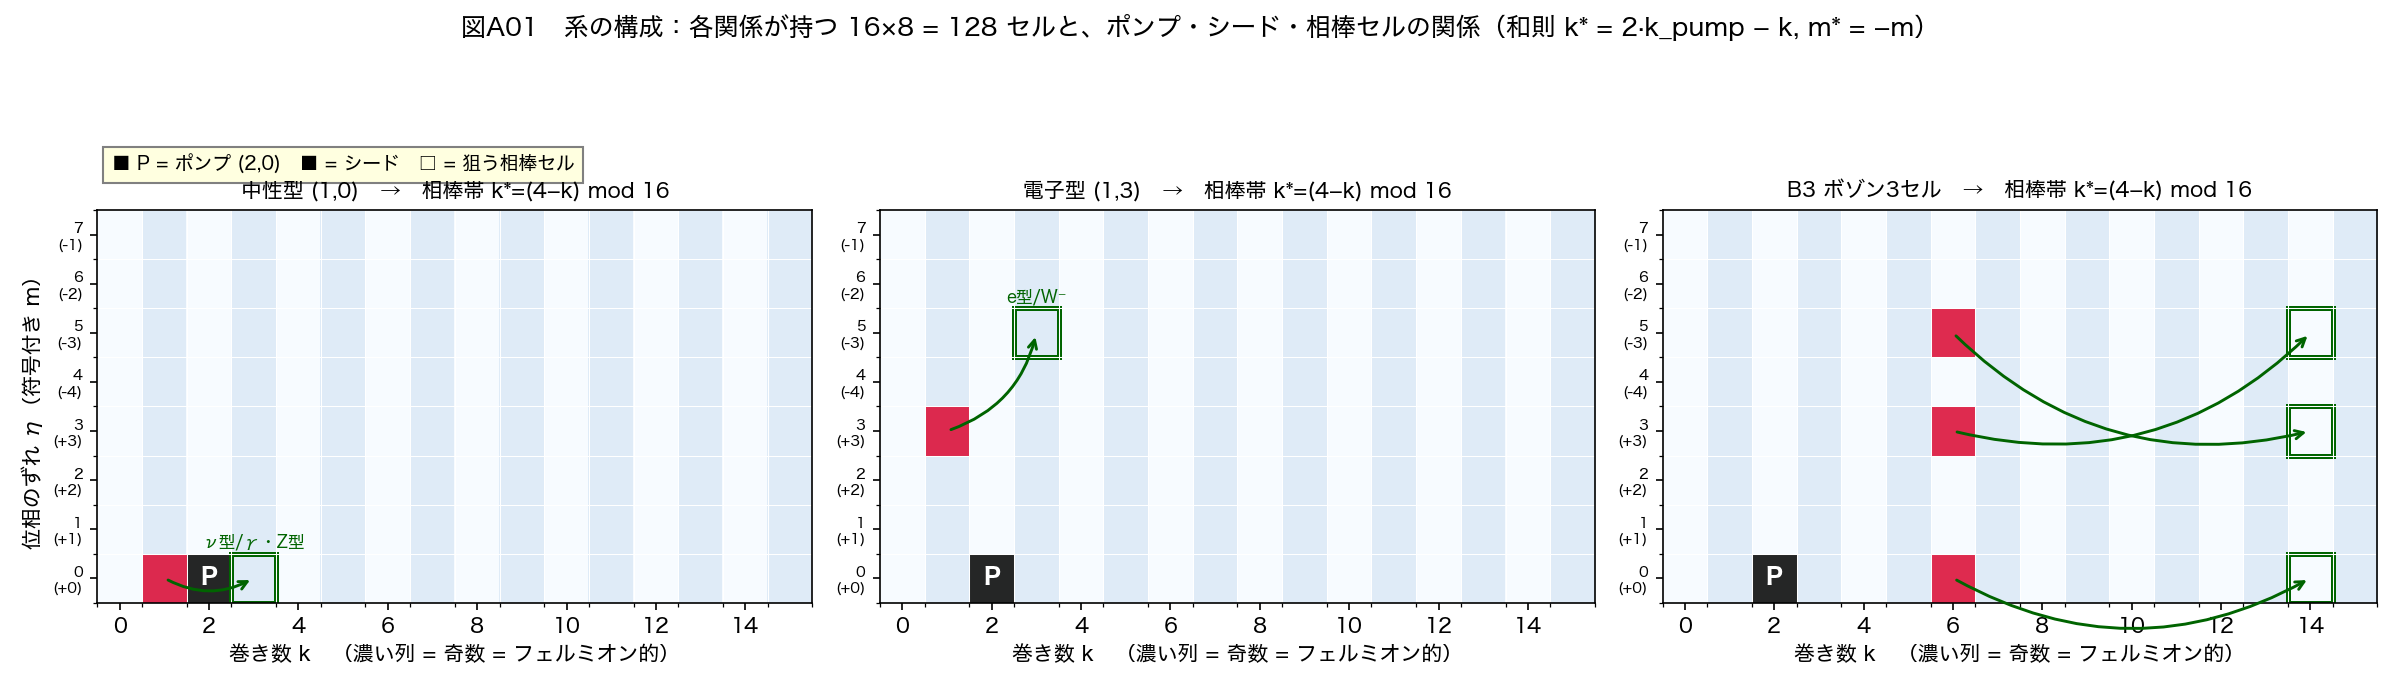
\includegraphics[keepaspectratio,alt={Figure 1　The system. The map of 128 locations carried by each relation, and the relation between the background oscillation (black), the seed (red) and the location it targets (green frame). Dark columns are odd bands.}]{figA01_lattice_and_seeds_v1.png}}

\textbf{Figure 1　The system. The map of 128 locations carried by each
relation, and the relation between the background oscillation (black),
the seed (red) and the location it targets (green frame). Dark columns
are odd bands.}

\subsubsection{The background oscillation and the
seed}\label{the-background-oscillation-and-the-seed}

Before a run starts, a wave of large amplitude is placed at location (k
= 2, m = 0). This is the \textbf{background oscillation}. It is common
to every condition, including the ``no seed'' case below. \textbf{It is
because of this background oscillation that inflation-like expansion
occurs even without a seed.}

On top of that, adding a small amplitude at specified locations is
called \textbf{seeding}. The magnitude added is the \textbf{seed
strength}, and the set of locations is the \textbf{seed placement}.

\subsubsection{Updates, and the count kept from
outside}\label{updates-and-the-count-kept-from-outside}

The system repeats discrete updates. \textbf{There are no seconds in
this paper; all time is measured in numbers of updates.} That count is a
scale we keep from outside; it is not inside the system.

One update has two halves. The first forms, for each relation, the
\textbf{sum of all 128 values taken as complex numbers}, decides a
rotation from the argument of that sum, and \textbf{applies the same
rotation to all 128 locations}. The second half is the interaction in
which three waves meet and make another.
\pandocbounded{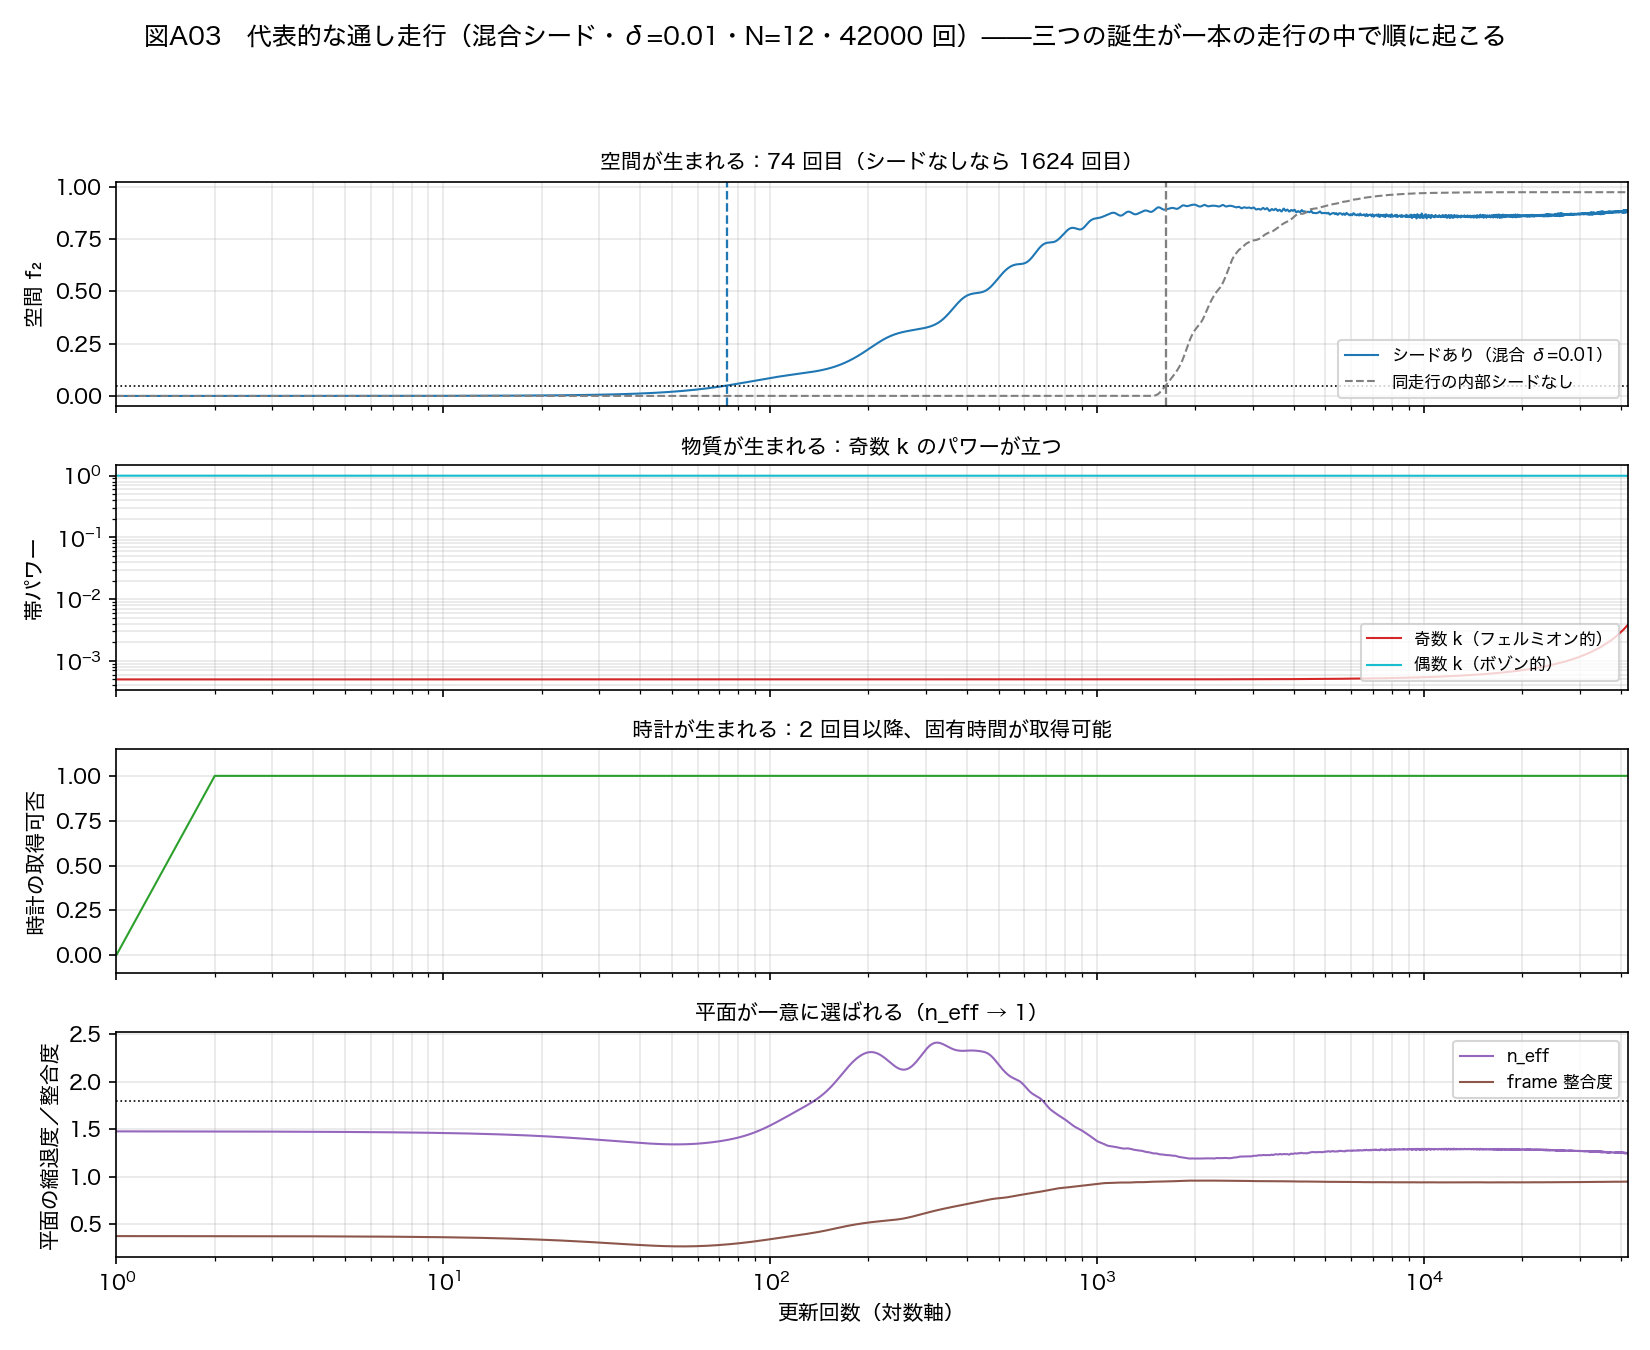
\includegraphics[keepaspectratio,alt={Figure 2　One representative run (mixed 8 locations, strength 0.01, resolution 12, 42000 updates). Space, matter and the clock are born in this order, and the plane finally settles on one.}]{figA03_full_run_example_v1.png}}

\textbf{Figure 2　One representative run (mixed 8 locations, strength
0.01, resolution 12, 42000 updates). Space, matter and the clock are
born in this order, and the plane finally settles on one.}

\subsubsection{The clock --- the time the system has of its
own}\label{the-clock-the-time-the-system-has-of-its-own}

As the system develops, it reaches a state in which \textbf{the whole
turns by a constant angle without changing shape}. Once that happens,
one can read from the state itself how many degrees it turned per
update. \textbf{That is the tick of time for the system, and in this
paper it is called the clock.}

Two conditions must hold for it to be readable: the overlap with the
immediately preceding state must exceed a floor, and the amplitude of
the component carrying the rotation must exceed a floor. The first
update at which both hold is when the \textbf{clock is born}.

\textbf{The count of updates kept from outside and this clock are
different things.} ``The clock is born at the 2nd update'' means that
after two updates on the outside scale, a tick of time has appeared
inside the system.

\subsubsection{The condensate}\label{the-condensate}

At the location where the background oscillation sits, the phases of the
gathered values align so that \textbf{squaring them and adding gives
zero} (they cancel). This state is called the \textbf{condensate}.
Particle-like waves are born on top of this lump. Here we say the
condensate exists when the residue of that cancellation is below 10⁻⁵.

\subsubsection{The third direction}\label{the-third-direction}

The distribution of the background oscillation initially lies within a
single plane. When a component growing outside that plane appears, a
\textbf{third direction} stands up. The first update at which the
fraction outside exceeds 5\% is when \textbf{space is born}.

But ``having grown outside'' does not fix the direction. If two or more
planes compete as the plane to grow out of, there is no telling which to
take as reference. We measure separately the degree to which one plane
is singled out, and when that exceeds a fixed value we say \textbf{the
third direction is determined}.
\pandocbounded{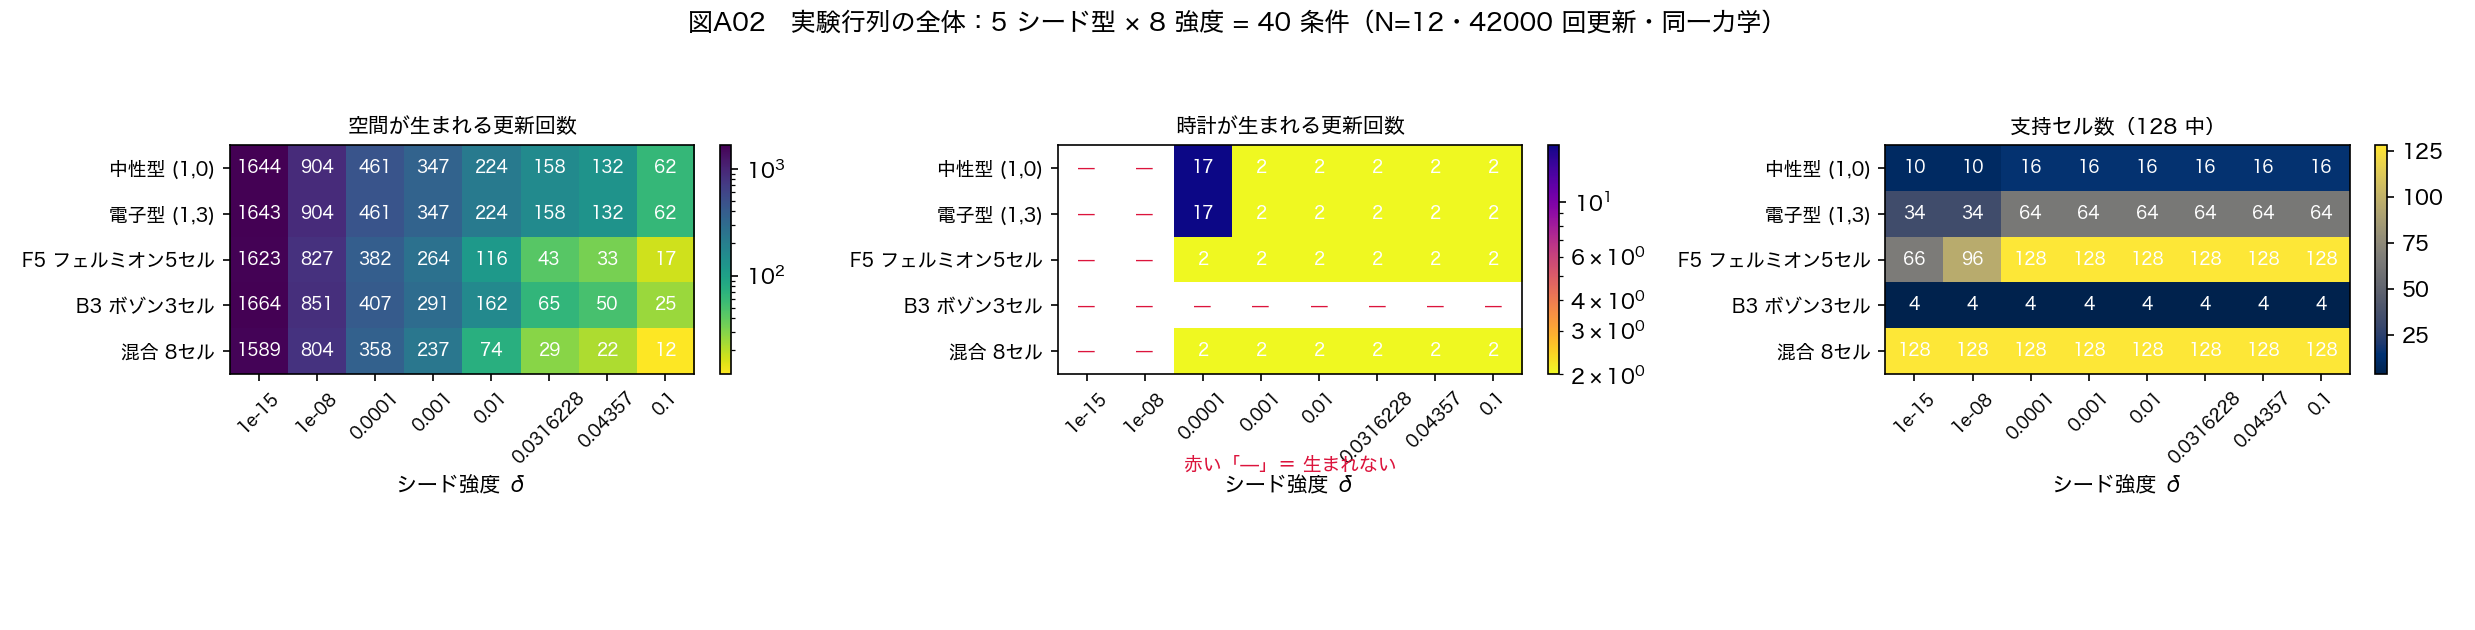
\includegraphics[keepaspectratio,alt={Figure 3　The whole main experiment. 5 seed placements × 8 strengths = 40 conditions, run with identical dynamics, resolution and number of updates. A red dash means not born.}]{figA02_experiment_matrix_v1.png}}

\textbf{Figure 3　The whole main experiment. 5 seed placements × 8
strengths = 40 conditions, run with identical dynamics, resolution and
number of updates. A red dash means not born.}

\begin{center}\rule{0.5\linewidth}{0.5pt}\end{center}

\subsection{1) The form of the seed gives partial control over which
kind of particle is
born}\label{the-form-of-the-seed-gives-partial-control-over-which-kind-of-particle-is-born}

Keeping the winding number k of the first direction fixed, we compared
\textbf{two seeds differing only in the winding number m of the second
direction}, placed with the same strength. One targets a partner that is
an uncharged wave (neutrino type); the other targets a partner that is
an electron-type wave.

The number of updates at which inflation starts, and the number at which
the clock is born, \textbf{agreed exactly for 7 of the 8 strengths}.
They differed by a single update only at the weakest strength, where the
run is indistinguishable from the no-seed case.

\textbf{Even so, the locations occupied by the resulting waves split
into 16 and 64.} For the electron type the pattern is a checkerboard:
when the first winding number is even so is the second, and when the
first is odd so is the second.

That is, \textbf{``when it is born'' and ``what is born'' are decided
separately}. The former is insensitive to the seed placement; the latter
is decided by it.
\pandocbounded{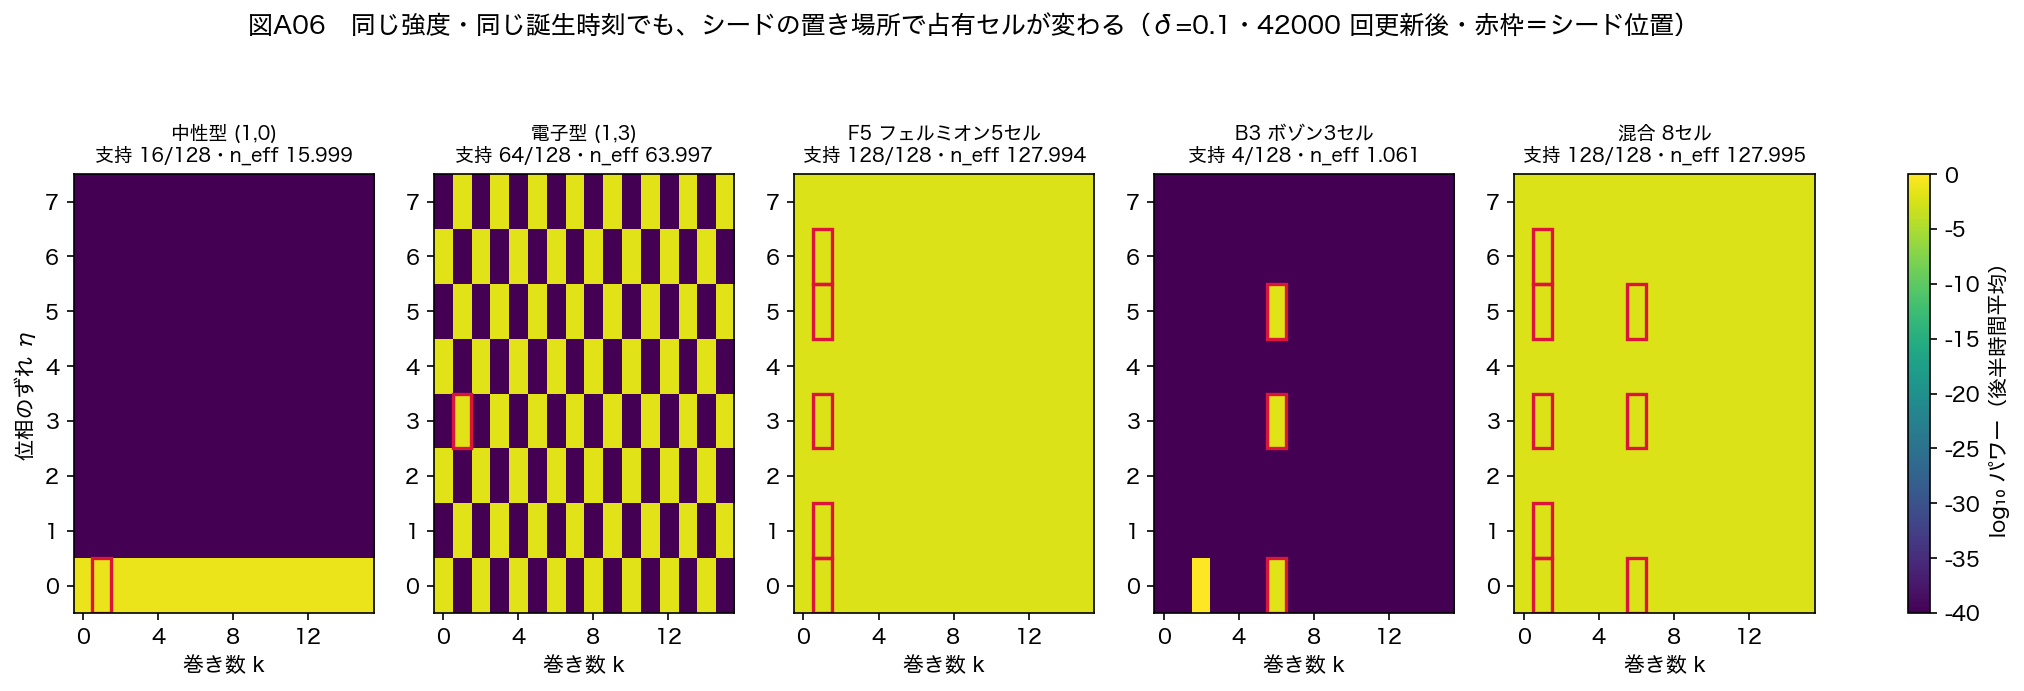
\includegraphics[keepaspectratio,alt={Figure 4　Locations occupied, for five seed placements (strength 0.1, after 42000 updates). Red frames mark the seed. The neutrino type occupies 16, the electron type a checkerboard of 64, and the even-band-only seed just 4.}]{figA06_support_structure_v1.png}}

\textbf{Figure 4　Locations occupied, for five seed placements (strength
0.1, after 42000 updates). Red frames mark the seed. The neutrino type
occupies 16, the electron type a checkerboard of 64, and the
even-band-only seed just 4.}

\subsubsection{Being born as intended happens only at intermediate
strength}\label{being-born-as-intended-happens-only-at-intermediate-strength}

Dividing the power at the targeted location by the power at non-targeted
locations measures how concentrated the result is at the target.

{\def\LTcaptype{none} % do not increment counter
\begin{longtable}[]{@{}lrrrrr@{}}
\toprule\noalign{}
Seed strength & 10⁻⁸ & 10⁻⁴ & \textbf{10⁻³} & 10⁻² & 0.03 and above \\
\midrule\noalign{}
\endhead
\bottomrule\noalign{}
\endlastfoot
Concentration & ≈ 0 & 0.009 & \textbf{10⁴} & 2×10³ & 0.08 \\
\end{longtable}
}

\textbf{If the seed is too strong the wave spreads over all 128
locations and the aim stops working.} The aim works best near strength
10⁻³, where concentration at the target reaches ten thousand-fold;
increasing the strength drops it by six orders of magnitude.

This concentration also varies by a factor of 120 with resolution (57 at
N = 3, 0.47 at N = 20).
\pandocbounded{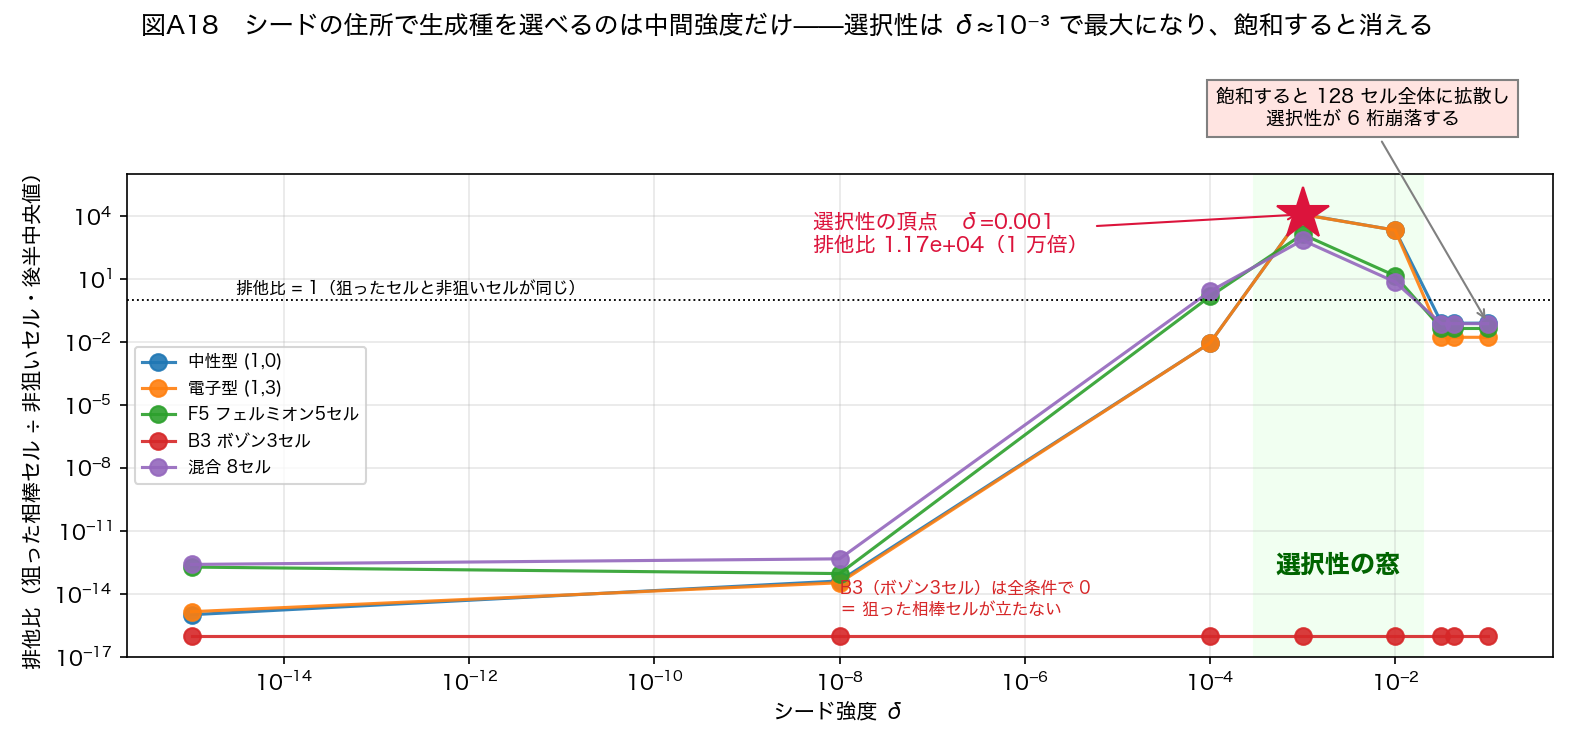
\includegraphics[keepaspectratio,alt={Figure 5　Concentration at the targeted location peaks near strength 10⁻³ and falls by six orders of magnitude as the seed is strengthened.}]{figA18_selectivity_window_v1.png}}

\textbf{Figure 5　Concentration at the targeted location peaks near
strength 10⁻³ and falls by six orders of magnitude as the seed is
strengthened.}

\begin{figure}
\centering
\pandocbounded{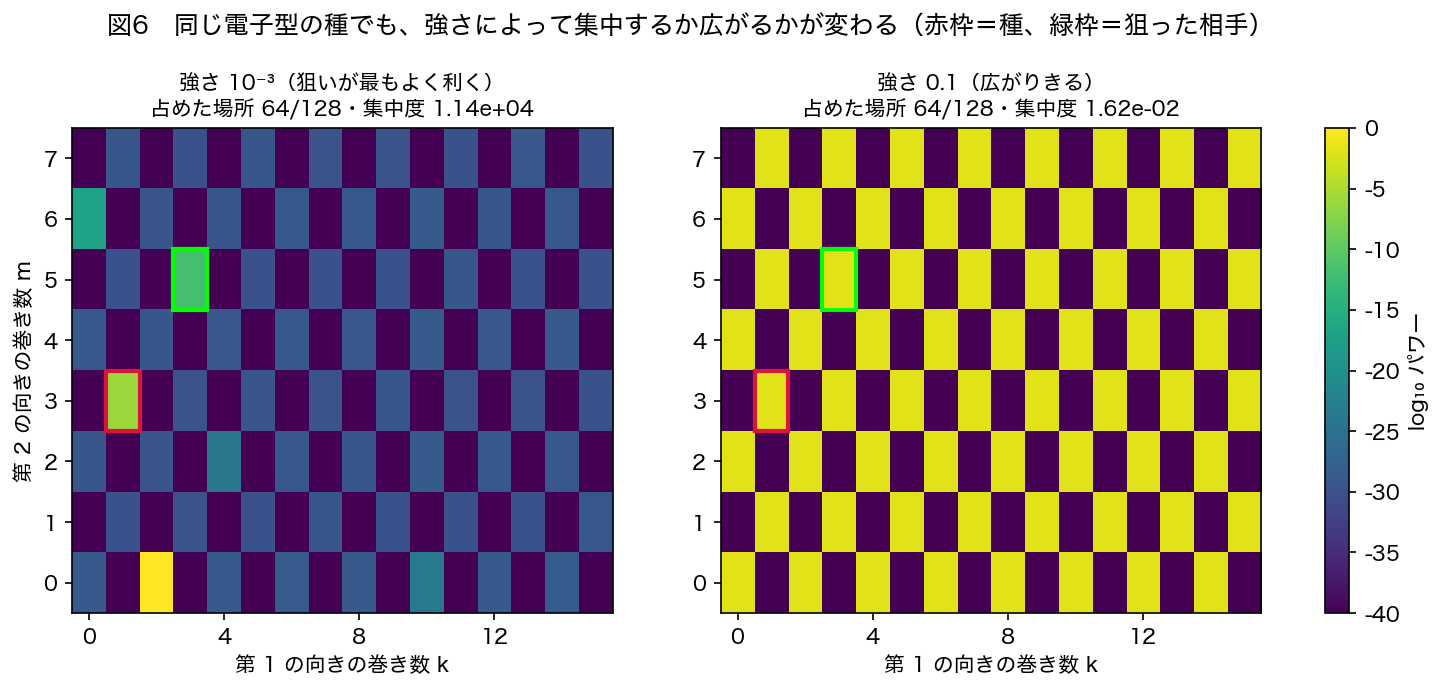
\includegraphics[keepaspectratio,alt={Figure 6　The map of 128 locations when concentrated (strength 10⁻³) and when fully spread (strength 0.1), for the same electron-type seed.}]{figA06b_ledger_pair_v1.png}}
\caption{Figure 6　The map of 128 locations when concentrated (strength
10⁻³) and when fully spread (strength 0.1), for the same electron-type
seed.}
\end{figure}

\textbf{Figure 6　The map of 128 locations when concentrated (strength
10⁻³) and when fully spread (strength 0.1), for the same electron-type
seed.}

\begin{center}\rule{0.5\linewidth}{0.5pt}\end{center}

\subsection{2) The seed amplitude appears to have a window, but that
appearance is created by the length of the
observation}\label{the-seed-amplitude-appears-to-have-a-window-but-that-appearance-is-created-by-the-length-of-the-observation}

If one looks only as far as 42000 updates, it appears that too weak a
seed yields inflation and three directions but no particle-like wave,
that a stronger seed yields particle-like waves, and that strengthening
further has no additional effect.

However, when the run was extended to 300000 updates, \textbf{at
strength 10⁻², where nothing appeared to happen within 42000 updates,
particle-like waves rose all at once at update 262,751}. It was not that
it had no effect; it took time to take effect.

{\def\LTcaptype{none} % do not increment counter
\begin{longtable}[]{@{}
  >{\raggedright\arraybackslash}p{(\linewidth - 10\tabcolsep) * \real{0.1304}}
  >{\raggedleft\arraybackslash}p{(\linewidth - 10\tabcolsep) * \real{0.1739}}
  >{\raggedleft\arraybackslash}p{(\linewidth - 10\tabcolsep) * \real{0.1739}}
  >{\raggedleft\arraybackslash}p{(\linewidth - 10\tabcolsep) * \real{0.1739}}
  >{\raggedleft\arraybackslash}p{(\linewidth - 10\tabcolsep) * \real{0.1739}}
  >{\raggedleft\arraybackslash}p{(\linewidth - 10\tabcolsep) * \real{0.1739}}@{}}
\toprule\noalign{}
\begin{minipage}[b]{\linewidth}\raggedright
Seed strength
\end{minipage} & \begin{minipage}[b]{\linewidth}\raggedleft
10⁻³
\end{minipage} & \begin{minipage}[b]{\linewidth}\raggedleft
\textbf{10⁻²}
\end{minipage} & \begin{minipage}[b]{\linewidth}\raggedleft
0.03
\end{minipage} & \begin{minipage}[b]{\linewidth}\raggedleft
0.044
\end{minipage} & \begin{minipage}[b]{\linewidth}\raggedleft
0.1
\end{minipage} \\
\midrule\noalign{}
\endhead
\bottomrule\noalign{}
\endlastfoot
Updates until they finish appearing & not reached in 42000 &
\textbf{262,751} & 25,760 & 13,391 & 2,352 \\
\end{longtable}
}

Within the measured range no boundary strength appears; the data connect
smoothly through the following empirical law.

\begin{verbatim}
(updates until they finish appearing) ∝ (power placed on odd bands)^(−1.073)
goodness of fit R² = 0.996 (14 points)
\end{verbatim}

Extrapolating this law, the number of updates diverges as the power
placed on odd bands approaches zero. \textbf{Therefore, seen within any
finite observation time, an apparent lower bound must arise.} Indeed a
seed placed on no odd band at all (power exactly zero) never finishes,
at any strength.

However, \textbf{it has not been shown that every non-zero seed
necessarily finishes in the infinite-time limit.} What has been shown is
that what looked like a threshold at 42000 updates collapsed at 300000,
and that the 14 measurable points lie on this law.

Within the measured range, then, the strength of the seed does not
decide whether particle-like waves can form, but how long they take to
form.

The amount produced differs qualitatively before and after.

\begin{itemize}
\tightlist
\item
  Before, the amount on odd bands is \textbf{exactly what was put in}
  (the seed power itself)
\item
  After, \textbf{odd and even bands are roughly half and half}
\end{itemize}

The lower bound ``too weak a seed yields no particle-like wave'' is
likewise likely an artefact of the observation time. A long run is
needed to check this (not done).
\pandocbounded{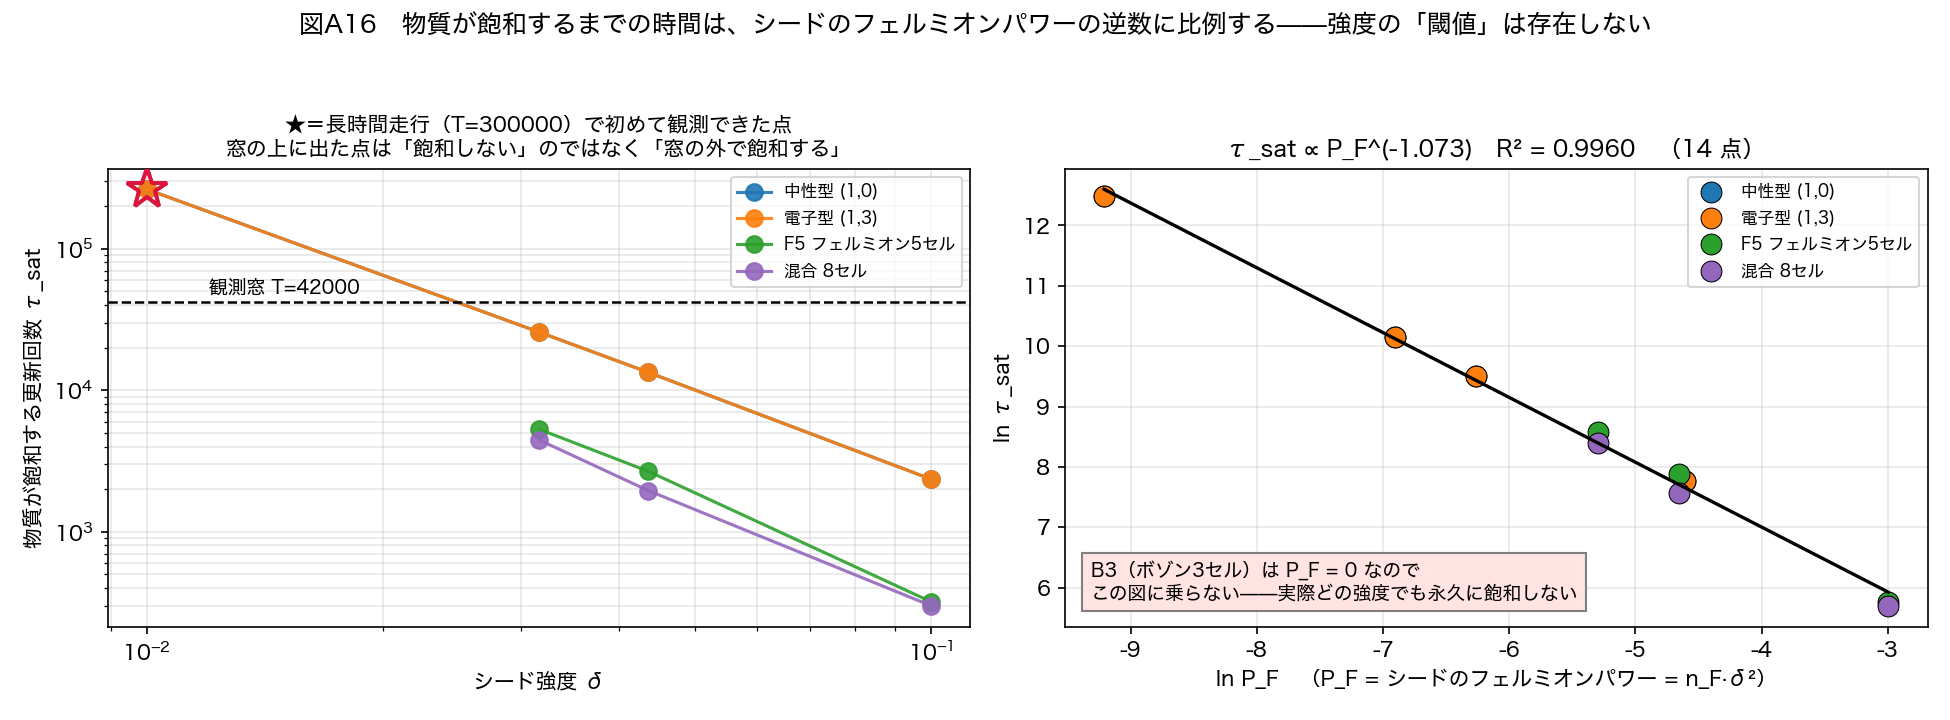
\includegraphics[keepaspectratio,alt={Figure 7　Updates until the particle-like waves finish appearing. Stars mark points that only the 300000-update runs could reach. Points above the 42000 line do not fail to finish; they finish outside that line. Right: the same data against the power placed on odd bands.}]{figA16_saturation_power_law_v1.png}}

\textbf{Figure 7　Updates until the particle-like waves finish
appearing. Stars mark points that only the 300000-update runs could
reach. Points above the 42000 line do not fail to finish; they finish
outside that line. Right: the same data against the power placed on odd
bands.}

\begin{figure}
\centering
\pandocbounded{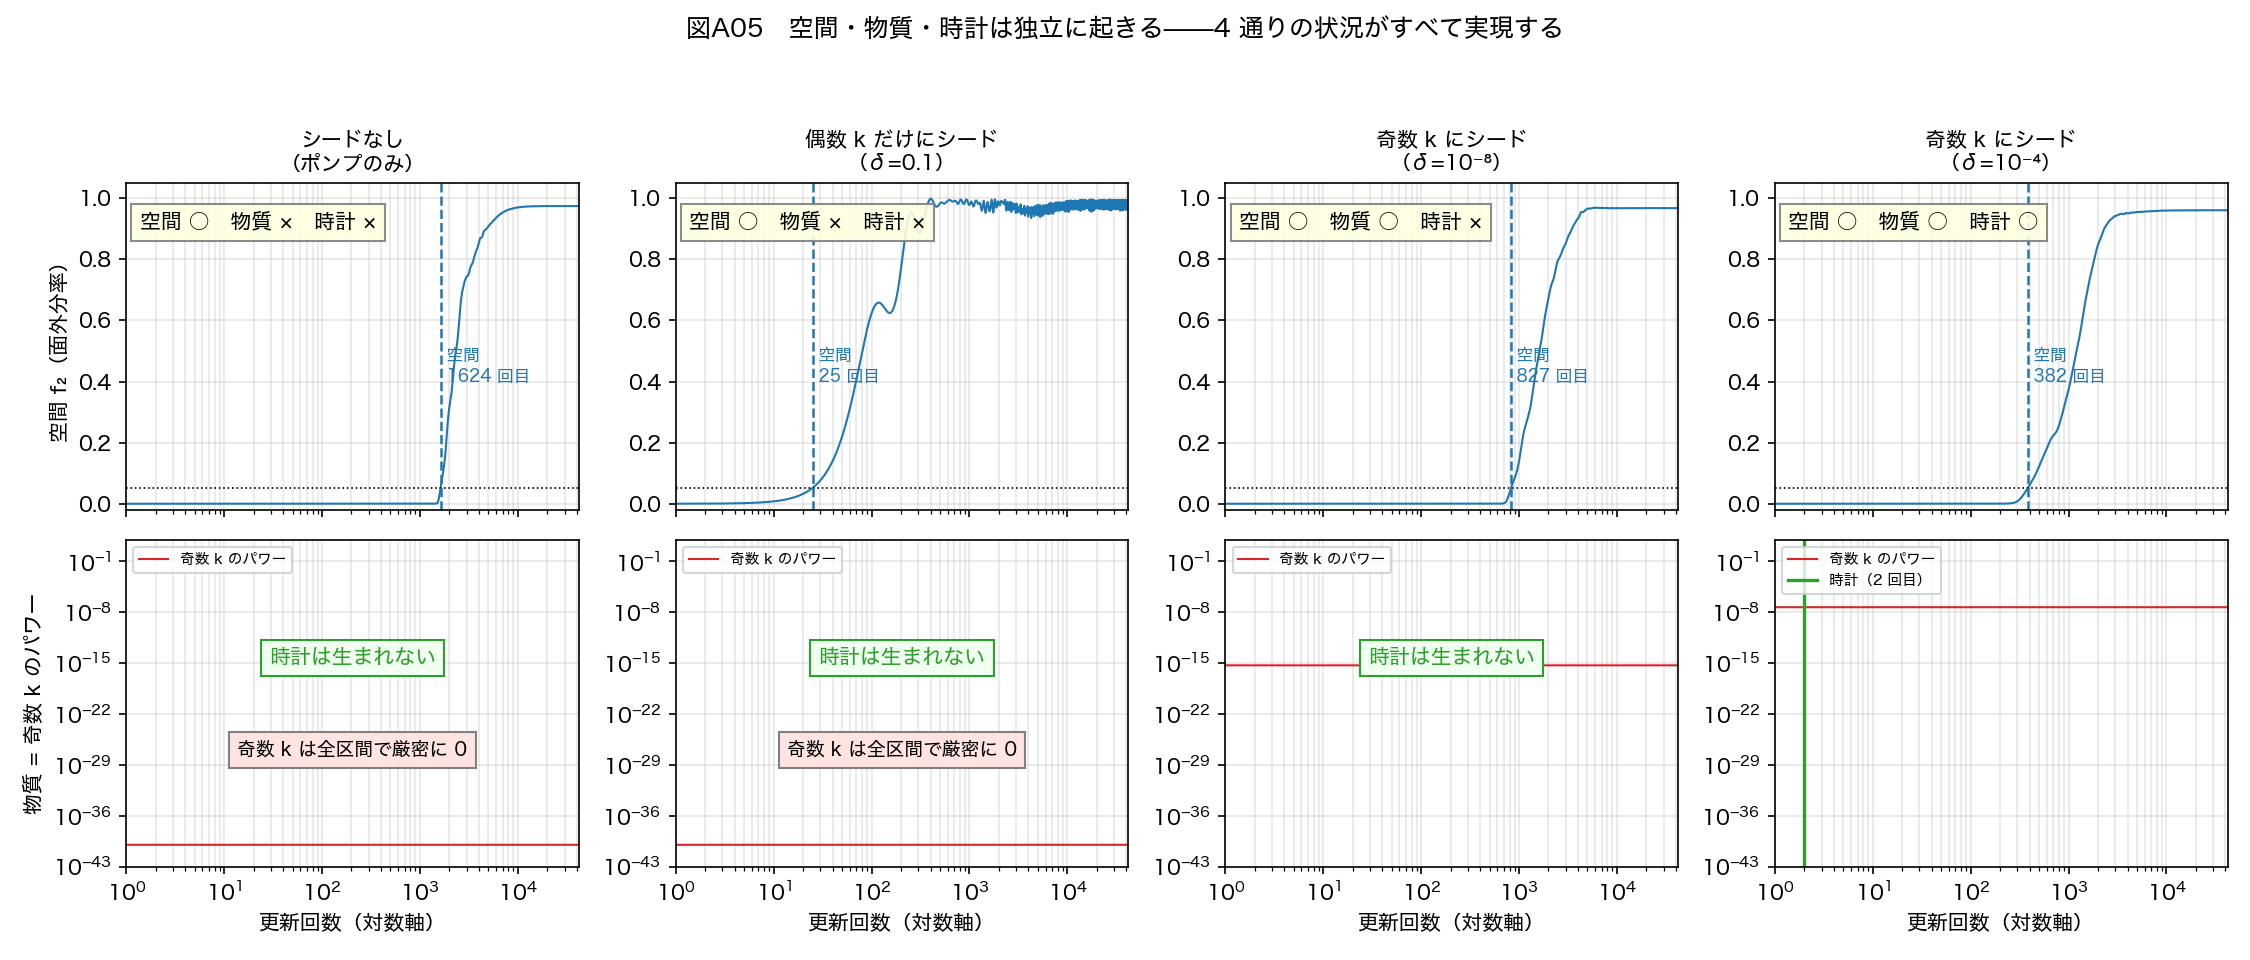
\includegraphics[keepaspectratio,alt={Figure 8　Space, matter and the clock do not share a birth condition. All four combinations occur.}]{figA05_three_births_v1.png}}
\caption{Figure 8　Space, matter and the clock do not share a birth
condition. All four combinations occur.}
\end{figure}

\textbf{Figure 8　Space, matter and the clock do not share a birth
condition. All four combinations occur.}

\begin{center}\rule{0.5\linewidth}{0.5pt}\end{center}

\subsection{3) The strength of the seed changes the run-up to the onset
of
inflation}\label{the-strength-of-the-seed-changes-the-run-up-to-the-onset-of-inflation}

The run-up shortens in proportion to the logarithm of the seed strength.

\begin{verbatim}
run-up = 9.892 − 48.611 × ln(magnitude of the seed summed as complex numbers)
goodness of fit R² = 0.99987
\end{verbatim}

What matters here is \textbf{not the total power of the seed but the
magnitude obtained by adding the seed as complex numbers}. Organised by
total power instead, the scatter worsens by a factor of 7.7.

This follows from the update procedure. The first half of an update
\textbf{looks only at the sum of the 128 values taken as complex
numbers} and applies the same rotation to every location. Two initial
states with the same sum are therefore indistinguishable to it.

This was tested directly. Without changing the seed's power or placement
at all, the \textbf{phases were arranged to cancel}, so that only the
sum becomes zero. It was then predicted, \textbf{before measuring}, that
the result would agree --- down to the number of updates --- with the
case having no seed on even bands. \textbf{All four strengths hit
exactly.}

{\def\LTcaptype{none} % do not increment counter
\begin{longtable}[]{@{}
  >{\raggedleft\arraybackslash}p{(\linewidth - 6\tabcolsep) * \real{0.2500}}
  >{\raggedleft\arraybackslash}p{(\linewidth - 6\tabcolsep) * \real{0.2500}}
  >{\raggedleft\arraybackslash}p{(\linewidth - 6\tabcolsep) * \real{0.2500}}
  >{\raggedleft\arraybackslash}p{(\linewidth - 6\tabcolsep) * \real{0.2500}}@{}}
\toprule\noalign{}
\begin{minipage}[b]{\linewidth}\raggedleft
Seed strength
\end{minipage} & \begin{minipage}[b]{\linewidth}\raggedleft
ordinary seed
\end{minipage} & \begin{minipage}[b]{\linewidth}\raggedleft
phase-cancelled seed
\end{minipage} & \begin{minipage}[b]{\linewidth}\raggedleft
no seed on even bands
\end{minipage} \\
\midrule\noalign{}
\endhead
\bottomrule\noalign{}
\endlastfoot
0.01 & 74 & \textbf{116} & 116 \\
0.03 & 29 & \textbf{43} & 43 \\
0.044 & 22 & \textbf{33} & 33 \\
0.1 & 12 & \textbf{17} & 17 \\
\end{longtable}
}

\begin{figure}
\centering
\pandocbounded{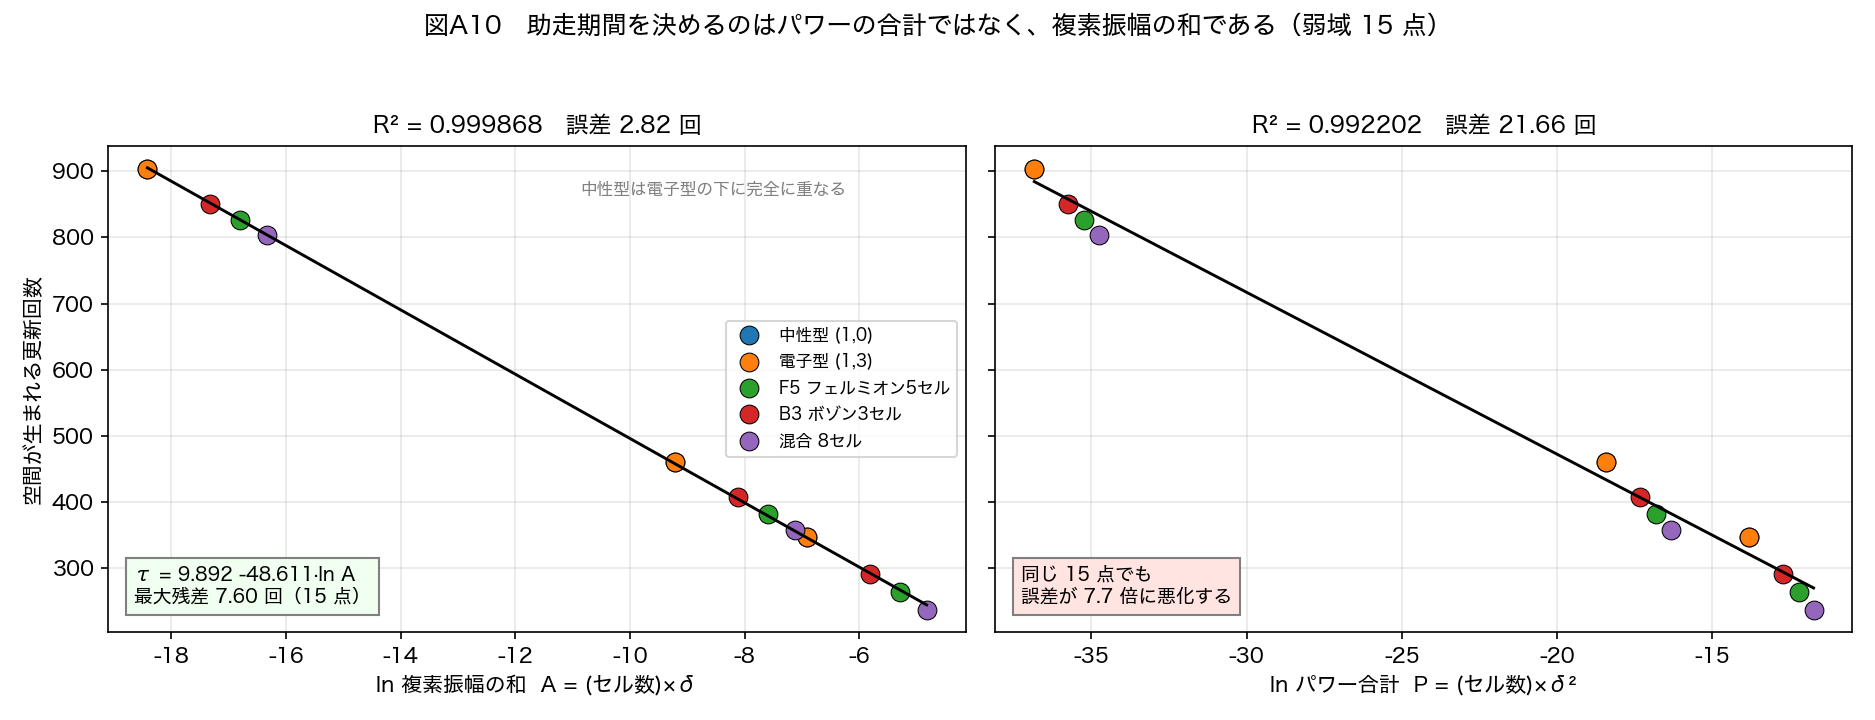
\includegraphics[keepaspectratio,alt={Figure 9　The run-up. Left: organised by the seed summed as complex numbers. Right: the same 15 points organised by total power.}]{figA10_runup_log_law_v1.png}}
\caption{Figure 9　The run-up. Left: organised by the seed summed as
complex numbers. Right: the same 15 points organised by total power.}
\end{figure}

\textbf{Figure 9　The run-up. Left: organised by the seed summed as
complex numbers. Right: the same 15 points organised by total power.}

\begin{figure}
\centering
\pandocbounded{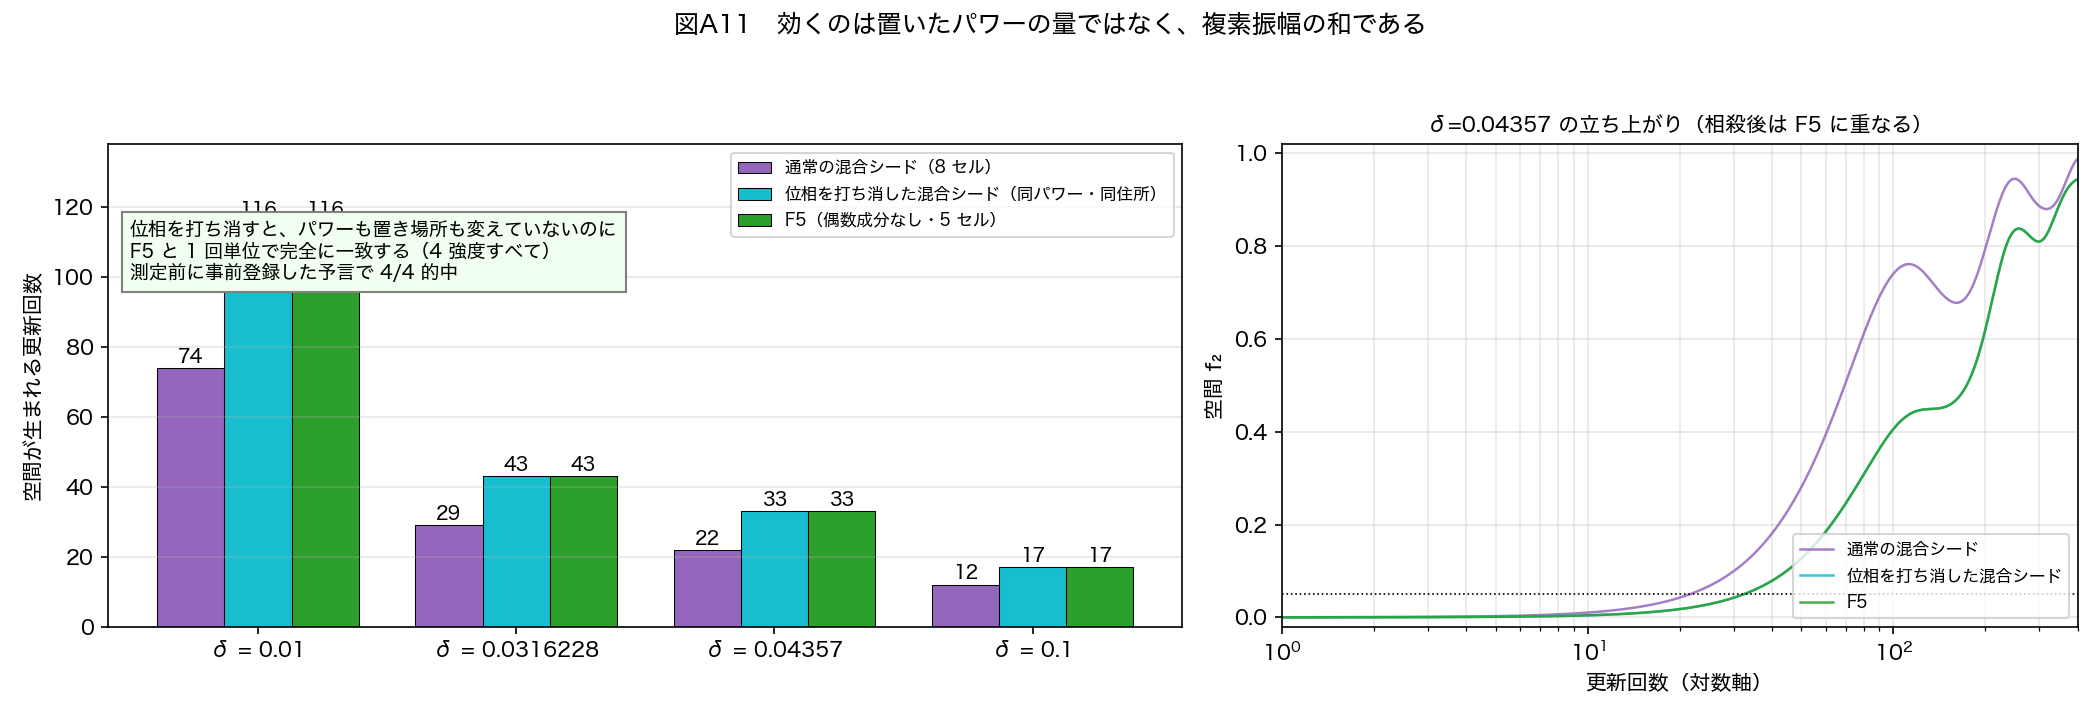
\includegraphics[keepaspectratio,alt={Figure 10　The phase-cancellation control. Without changing power or placement, the result agrees update for update with the case having no seed on even bands.}]{figA11_phase_cancellation_v1.png}}
\caption{Figure 10　The phase-cancellation control. Without changing
power or placement, the result agrees update for update with the case
having no seed on even bands.}
\end{figure}

\textbf{Figure 10　The phase-cancellation control. Without changing
power or placement, the result agrees update for update with the case
having no seed on even bands.}

\subsubsection{This control experiment alone cannot separate the sum
from the sum of
squares}\label{this-control-experiment-alone-cannot-separate-the-sum-from-the-sum-of-squares}

The cancellation used a triple of equal amplitudes with phases 0, 2π/3
and 4π/3. That arrangement makes the complex sum zero, but \textbf{it
also makes the sum of squares zero} (both of order 10⁻¹⁵).

\textbf{This experiment alone therefore cannot tell whether the first
half of an update reads the ``sum'' or the ``sum of squares''.} The
paper says it is the sum because the update procedure itself uses only
the argument of the sum. The experiment is consistent with that, but it
does not on its own single out the sum.

To separate them one needs an arrangement whose sum is zero but whose
sum of squares is not (for example a pair with phase difference π). That
was not done here.

\subsubsection{The complex sum matters only for the
onset}\label{the-complex-sum-matters-only-for-the-onset}

The ``updates until the waves finish appearing'' of section 2 is instead
decided by total power. Two different rules of decision coexist in the
same system.

{\def\LTcaptype{none} % do not increment counter
\begin{longtable}[]{@{}
  >{\raggedright\arraybackslash}p{(\linewidth - 4\tabcolsep) * \real{0.3333}}
  >{\raggedright\arraybackslash}p{(\linewidth - 4\tabcolsep) * \real{0.3333}}
  >{\raggedright\arraybackslash}p{(\linewidth - 4\tabcolsep) * \real{0.3333}}@{}}
\toprule\noalign{}
\begin{minipage}[b]{\linewidth}\raggedright
What is observed
\end{minipage} & \begin{minipage}[b]{\linewidth}\raggedright
Decided by
\end{minipage} & \begin{minipage}[b]{\linewidth}\raggedright
Quantity that matters
\end{minipage} \\
\midrule\noalign{}
\endhead
\bottomrule\noalign{}
\endlastfoot
Onset of inflation & first half of an update & the \textbf{sum} taken as
complex numbers \\
Time when particle-like waves finish appearing & second half & the total
\textbf{power} \\
\end{longtable}
}

The first half looks only at the sum. The second is proportional to a
coefficient built from the ratio of odd-band to even-band power. Hence
the quantity that matters depends on which phenomenon is observed.

A seed placed only on even bands satisfies both at once. Its odd-band
power is zero, so the finishing time is infinite (and indeed it never
finishes at any strength), while its onset lies on the straight line of
the complex sum.
\pandocbounded{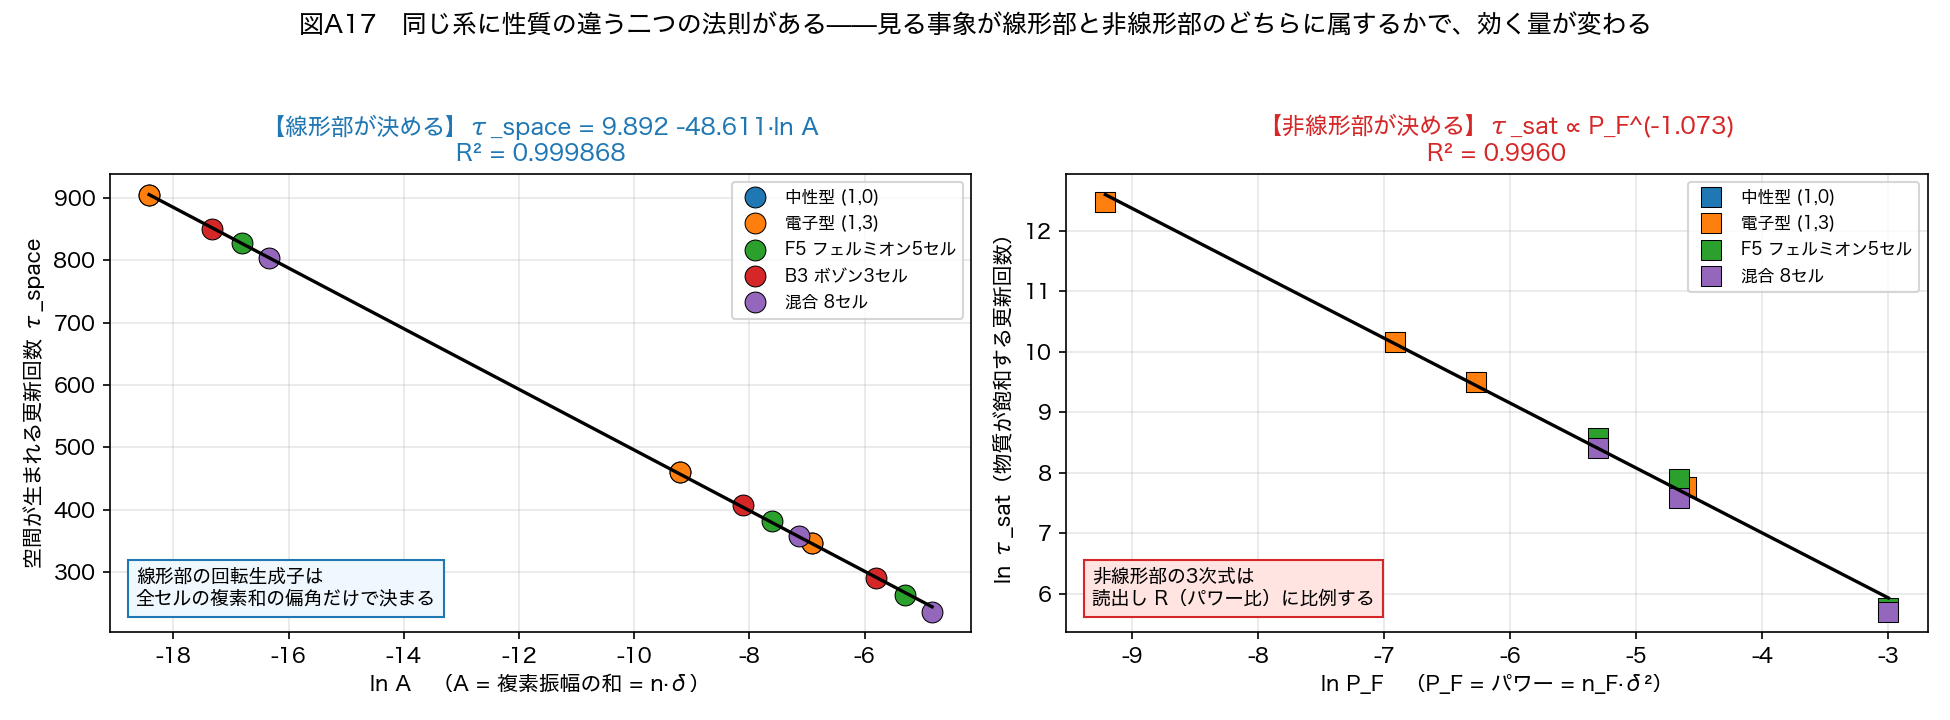
\includegraphics[keepaspectratio,alt={Figure 11　Two rules of decision in one system. Left: the onset, decided by the first half of an update. Right: the finishing time, decided by the second half.}]{figA17_two_laws_v1.png}}

\textbf{Figure 11　Two rules of decision in one system. Left: the onset,
decided by the first half of an update. Right: the finishing time,
decided by the second half.}

\begin{figure}
\centering
\pandocbounded{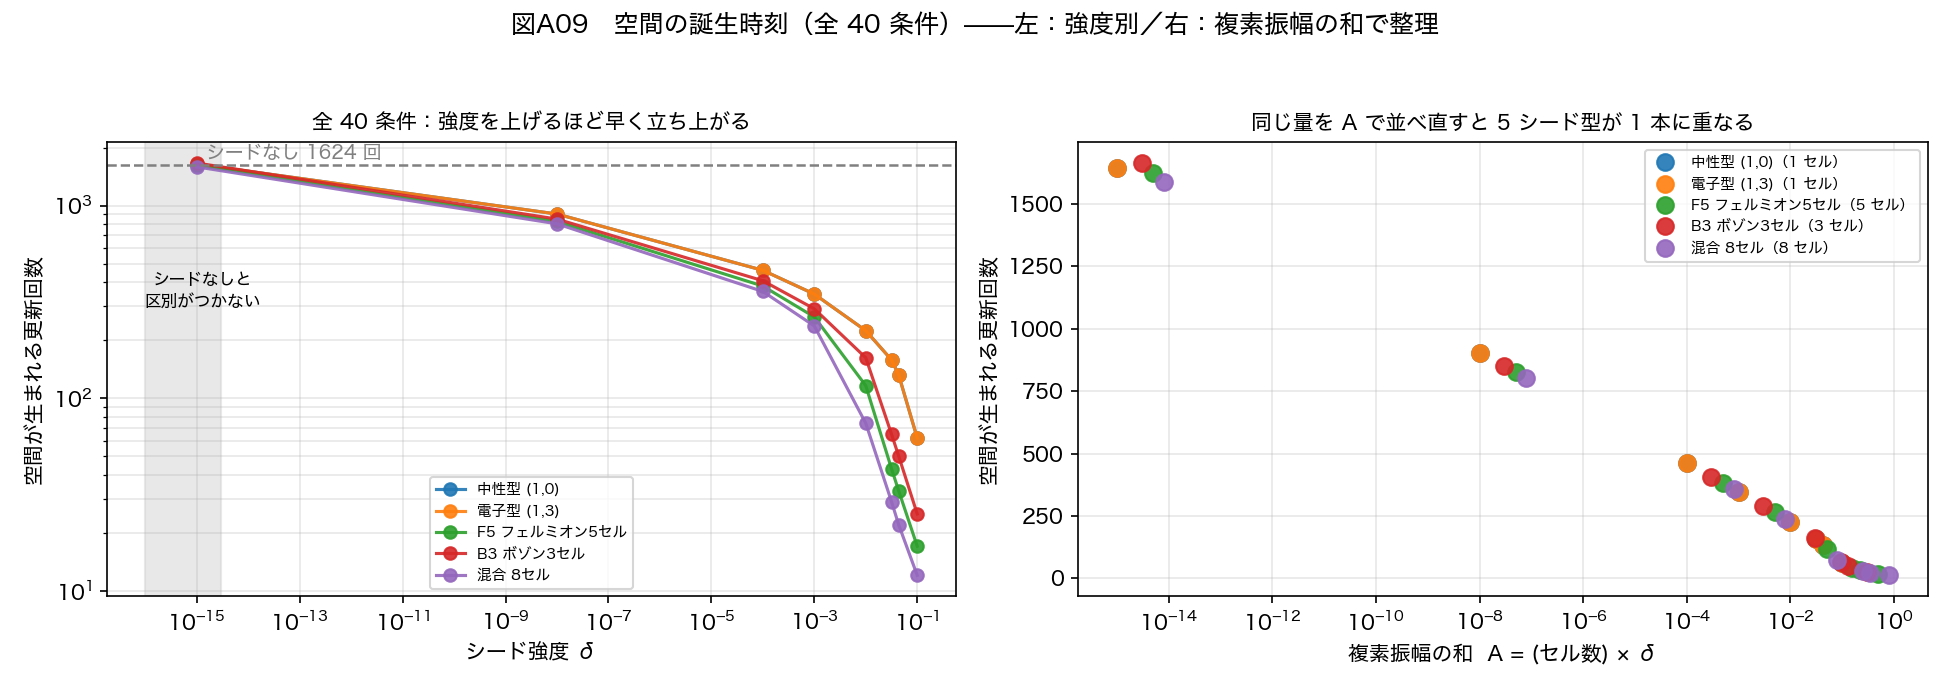
\includegraphics[keepaspectratio,alt={Figure 12　Updates to onset for all 40 conditions. Re-plotted against the seed summed as complex numbers (right), the five placements fall on one curve.}]{figA09_tau_space_all_conditions_v1.png}}
\caption{Figure 12　Updates to onset for all 40 conditions. Re-plotted
against the seed summed as complex numbers (right), the five placements
fall on one curve.}
\end{figure}

\textbf{Figure 12　Updates to onset for all 40 conditions. Re-plotted
against the seed summed as complex numbers (right), the five placements
fall on one curve.}

\begin{center}\rule{0.5\linewidth}{0.5pt}\end{center}

\subsection{4) There is a minimum resolution: at N = 1, 2 neither
inflation nor three directions
appeared}\label{there-is-a-minimum-resolution-at-n-1-2-neither-inflation-nor-three-directions-appeared}

At N = 1 there is not a single relation between points, and at N = 2
only one, so the system cannot be built at all.

\subsubsection{There are singular resolutions: at N = 3, 4 the third
direction is not
determined}\label{there-are-singular-resolutions-at-n-3-4-the-third-direction-is-not-determined}

\textbf{At N = 3 and N = 4 the planes compete and no single plane is
selected, so the third direction is not determined.} Three planes
compete at N = 3 and two at N = 4. Moreover this competition
\textbf{never settles; it keeps fluctuating over the whole run.} There
is no steady state.

N = 5 and 6 show yet another aspect: \textbf{quiet stretches alternate
with violently fluctuating ones.} Only from N = 7 upward does a single
plane dominate.

\textbf{At N = 8 and N = 10 the initial state itself could not be
built.} This, however, is because the implementation stops after one
failed attempt; it has not been confirmed that it is structurally
impossible (unverified).

\textbf{Seeding acts to resolve the competition.} Among the 16
resolutions that could be built, the number showing competition falls
from 8 with no seed, to 4 with a seed at one location, to 2 with seeds
at eight locations. \textbf{N = 3 and N = 4 alone cannot be resolved by
any amount of seeding.}

There is no relation of the kind ``resolutions that compete have longer
run-ups''. The two are separate properties.
\pandocbounded{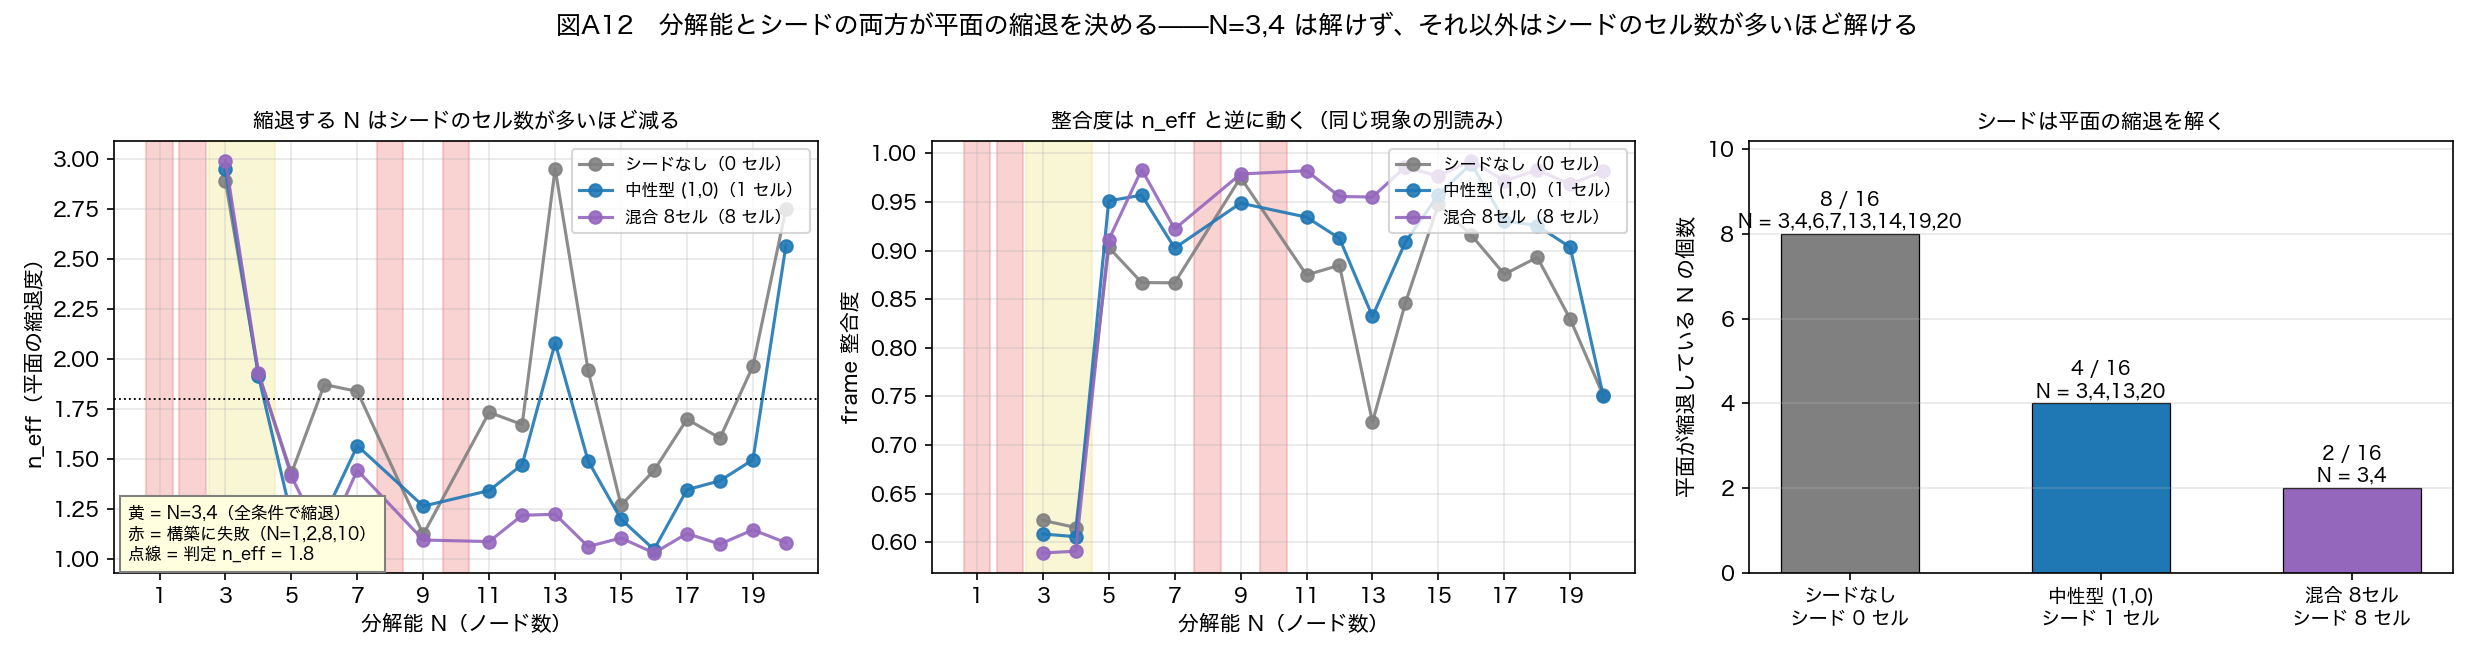
\includegraphics[keepaspectratio,alt={Figure 13　Competition between planes, by resolution and seed. Yellow marks N = 3, 4 (competing under every condition); red marks resolutions where the initial state could not be built. Right: the more seed locations, the fewer resolutions compete.}]{figA12_resolution_regimes_v1.png}}

\textbf{Figure 13　Competition between planes, by resolution and seed.
Yellow marks N = 3, 4 (competing under every condition); red marks
resolutions where the initial state could not be built. Right: the more
seed locations, the fewer resolutions compete.}

\begin{figure}
\centering
\pandocbounded{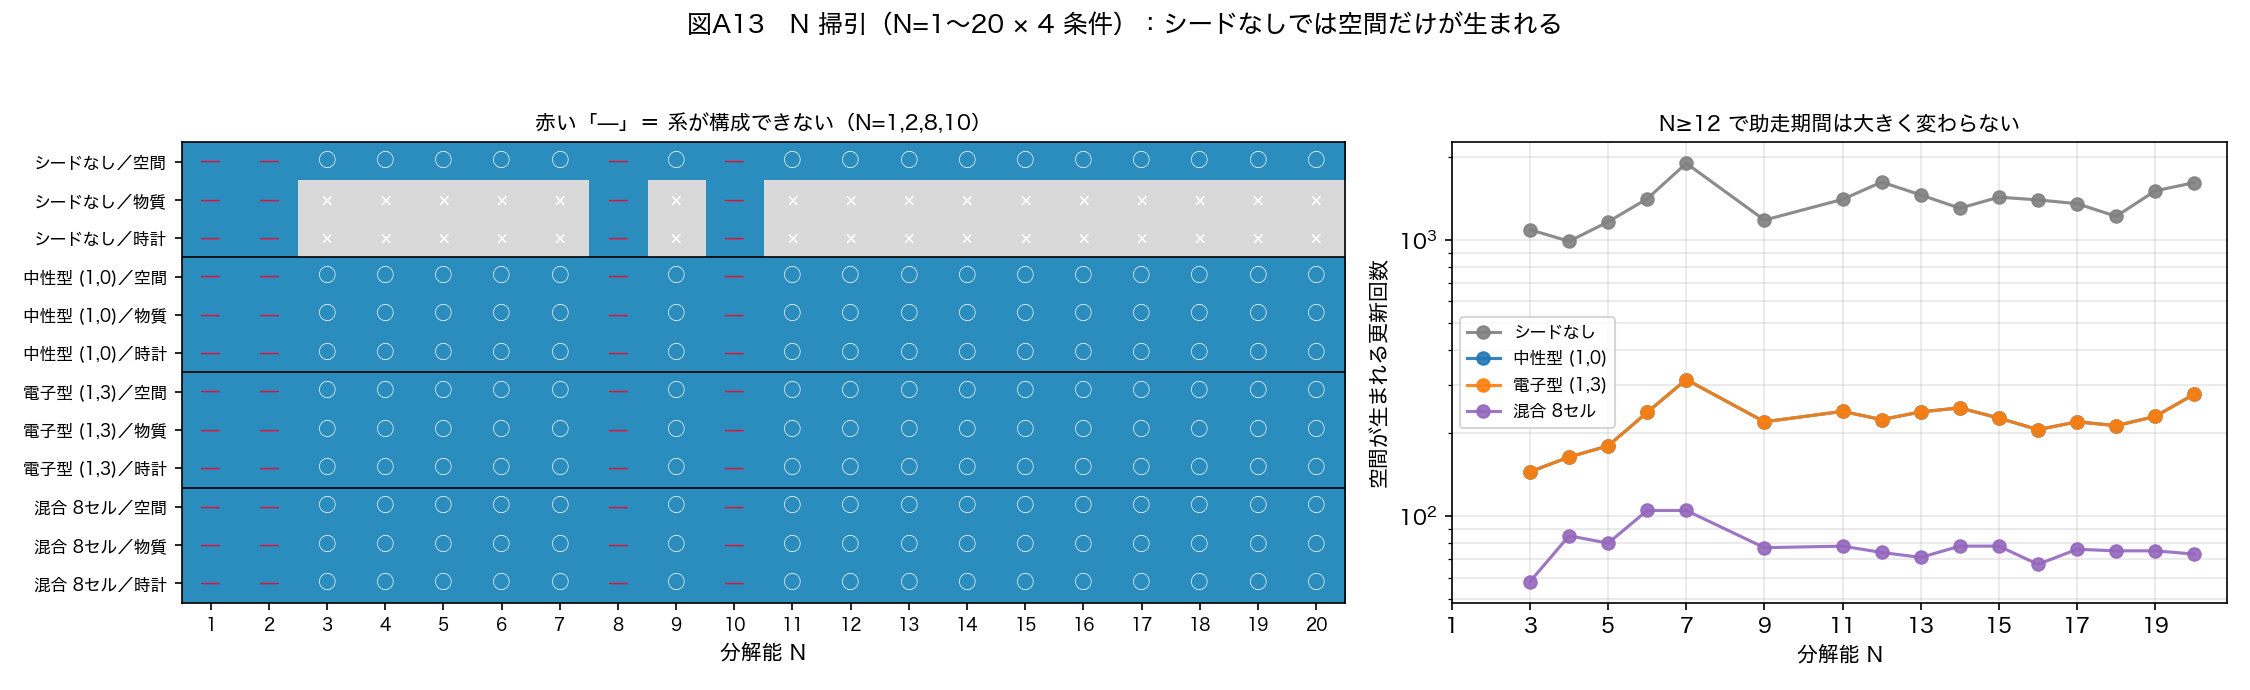
\includegraphics[keepaspectratio,alt={Figure 14　The judgements for four conditions over resolutions 1--20. In the no-seed rows only space is marked, with matter and the clock absent at every resolution.}]{figA13_nsweep_birth_matrix_v1.png}}
\caption{Figure 14　The judgements for four conditions over resolutions
1--20. In the no-seed rows only space is marked, with matter and the
clock absent at every resolution.}
\end{figure}

\textbf{Figure 14　The judgements for four conditions over resolutions
1--20. In the no-seed rows only space is marked, with matter and the
clock absent at every resolution.}

\subsubsection{Three anomalies that appear only at N =
4}\label{three-anomalies-that-appear-only-at-n-4}

\begin{enumerate}
\def\labelenumi{\arabic{enumi}.}
\tightlist
\item
  Two planes compete and the third direction is not determined
\item
  \textbf{The clock ticks 9.9 times faster than at other resolutions}
\item
  \textbf{It is the only resolution at which the readout crosses the
  special value 0.6972 reported in the previous paper}
\end{enumerate}

Examining all 126 runs, the only ones to exceed that value are
\textbf{the two runs with a single-location seed at N = 4}, reaching a
maximum of 0.8019. The neutrino type and the electron type agree to 12
digits on that value. The closest approach is 0.0000068 (0.001\% in
relative terms).

\textbf{But it only crosses; it does not stay.} The readout lies within
±0.001 of that value for \textbf{only 9 of the 42000 updates}. At N = 4
the system keeps fluctuating violently after the waves have finished
appearing, and the fluctuation happens to cross the value. At N = 12 the
maximum is 0.6786, short of that value by 2.7\%.
\pandocbounded{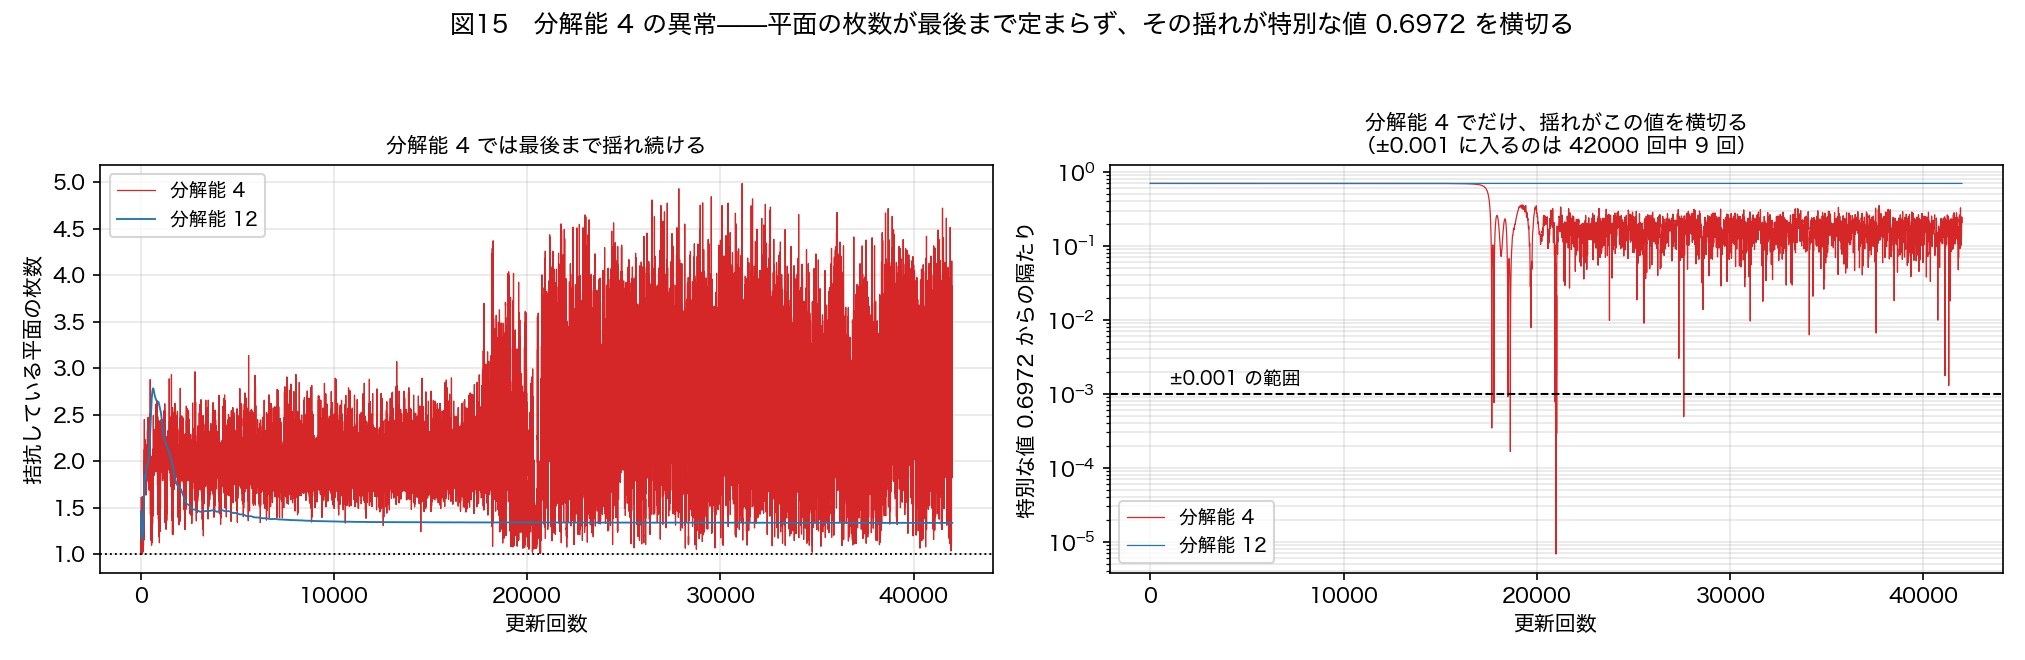
\includegraphics[keepaspectratio,alt={Figure 15　The anomaly at resolution 4. The number of competing planes never settles (left), and that fluctuation crosses the special value 0.6972 (right).}]{figA04b_N4_anomaly_v1.png}}

\textbf{Figure 15　The anomaly at resolution 4. The number of competing
planes never settles (left), and that fluctuation crosses the special
value 0.6972 (right).}

\subsubsection{From N ≥ 12 up to N = 20, tested, there was broadly no
large change of
behaviour}\label{from-n-12-up-to-n-20-tested-there-was-broadly-no-large-change-of-behaviour}

The run-up stays within 206--277 updates with no monotone trend.

\textbf{There are two exceptions.} Competition between planes reappears
at N = 13 and N = 20. In particular \textbf{at N = 20 the third
direction is not determined}.

\subsubsection{After the waves finish appearing, the plane stops being
determined
again}\label{after-the-waves-finish-appearing-the-plane-stops-being-determined-again}

``A single plane dominates from N = 7 upward'' refers to the state
before the particle-like waves finish appearing. Afterwards the number
of competing planes keeps fluctuating at every resolution.

\begin{center}\rule{0.5\linewidth}{0.5pt}\end{center}

\subsection{5) There are not four things that ``are born'' but six, and
a strong seed destroys the last
two}\label{there-are-not-four-things-that-are-born-but-six-and-a-strong-seed-destroys-the-last-two}

What the experiment judges is the following six.

Whether the system could be built / whether \textbf{space is born} (a
third direction stands up) / whether \textbf{matter is born} (waves
appear on odd bands) / whether \textbf{the clock is born} (the system
can read its own time) / whether \textbf{the third direction is
determined} / whether \textbf{the condensate exists}.

As the seed is strengthened, \textbf{the first four increase but the
last two are lost}.

{\def\LTcaptype{none} % do not increment counter
\begin{longtable}[]{@{}
  >{\raggedleft\arraybackslash}p{(\linewidth - 10\tabcolsep) * \real{0.1667}}
  >{\centering\arraybackslash}p{(\linewidth - 10\tabcolsep) * \real{0.1667}}
  >{\centering\arraybackslash}p{(\linewidth - 10\tabcolsep) * \real{0.1667}}
  >{\centering\arraybackslash}p{(\linewidth - 10\tabcolsep) * \real{0.1667}}
  >{\centering\arraybackslash}p{(\linewidth - 10\tabcolsep) * \real{0.1667}}
  >{\centering\arraybackslash}p{(\linewidth - 10\tabcolsep) * \real{0.1667}}@{}}
\toprule\noalign{}
\begin{minipage}[b]{\linewidth}\raggedleft
Seed strength
\end{minipage} & \begin{minipage}[b]{\linewidth}\centering
space
\end{minipage} & \begin{minipage}[b]{\linewidth}\centering
matter
\end{minipage} & \begin{minipage}[b]{\linewidth}\centering
clock
\end{minipage} & \begin{minipage}[b]{\linewidth}\centering
third direction determined
\end{minipage} & \begin{minipage}[b]{\linewidth}\centering
condensate
\end{minipage} \\
\midrule\noalign{}
\endhead
\bottomrule\noalign{}
\endlastfoot
10⁻¹⁵, 10⁻⁸ & ○ & ○ & \textbf{×} & ○ & ○ \\
10⁻⁴, 10⁻³ & ○ & ○ & ○ & ○ & ○ \\
10⁻² & ○ & ○ & ○ & ○ & \textbf{×} (with many seed locations) \\
0.03 and above & ○ & ○ & ○ & \textbf{×} & \textbf{×} \\
\end{longtable}
}

\textbf{A strong seed produces matter and a clock at the cost of the
certainty of the third direction and of the condensate.} Things do not
simply come into being; there is a trade.

Furthermore, extending the run to 300000 updates, \textbf{the condensate
is eventually destroyed even at strength 10⁻²}. That it looked intact at
42000 updates only means it had not yet been destroyed.
\pandocbounded{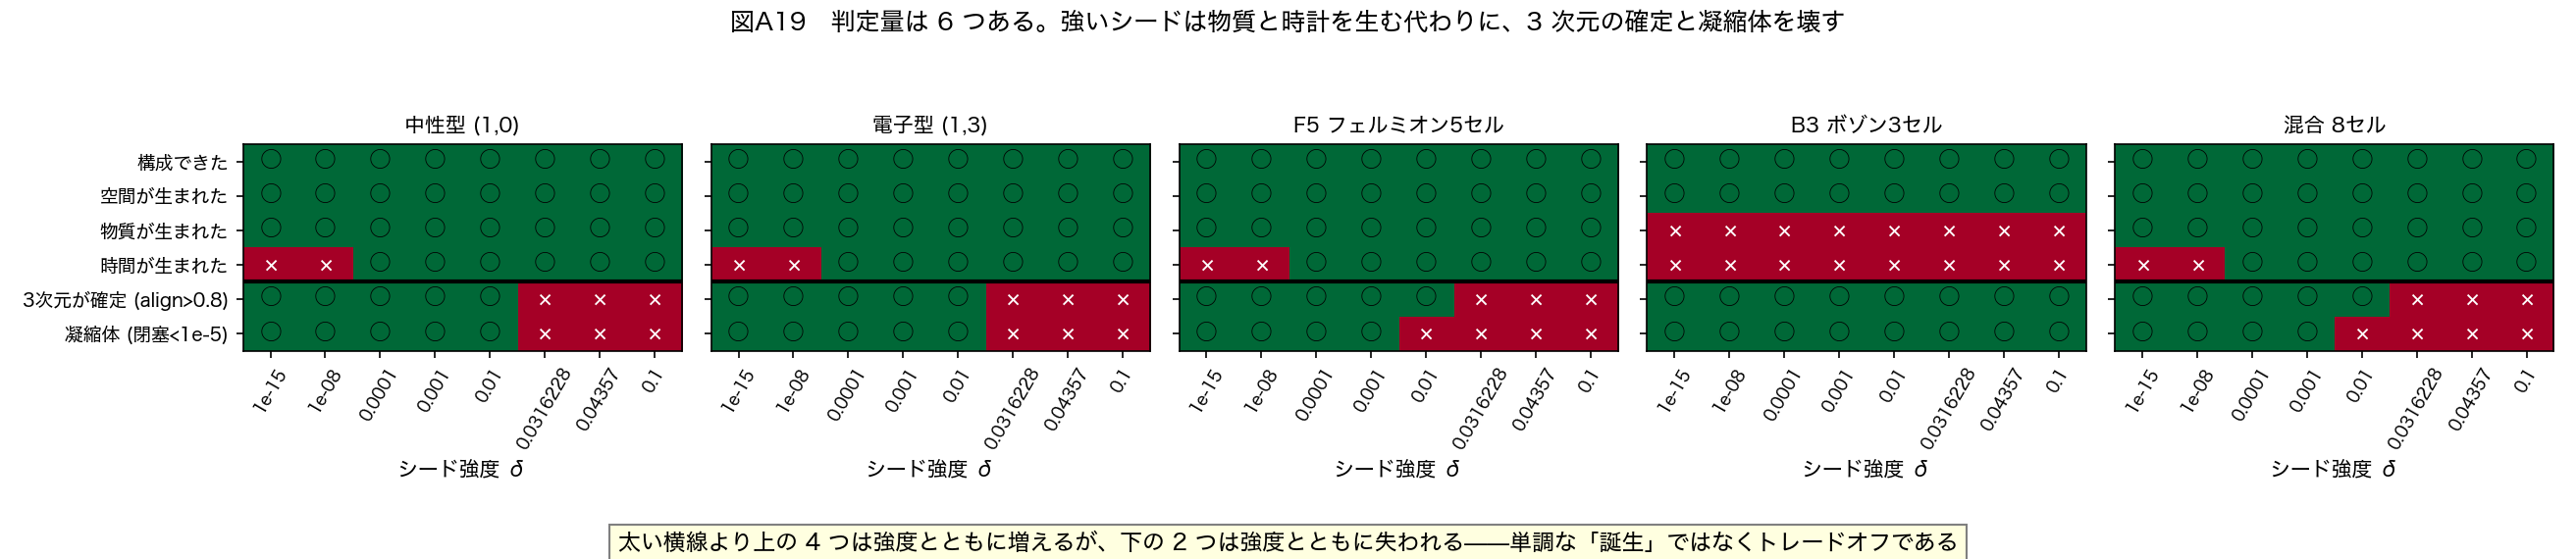
\includegraphics[keepaspectratio,alt={Figure 16　The six criteria. Above the thick line the first four increase with seed strength; below it the last two are lost.}]{figA19_six_criteria_tradeoff_v1.png}}

\textbf{Figure 16　The six criteria. Above the thick line the first four
increase with seed strength; below it the last two are lost.}

\begin{center}\rule{0.5\linewidth}{0.5pt}\end{center}

\subsection{6) With a seed on even bands only, the interaction itself
never occurs even
once}\label{with-a-seed-on-even-bands-only-the-interaction-itself-never-occurs-even-once}

With a seed on even bands only, \textbf{no wave whatsoever appears on
the odd bands}, over the whole of 42000 updates and all 8 strengths.
More than that, \textbf{only 2 of the 16 bands ever carry a wave} ---
the background oscillation and the seed itself --- and \textbf{not even
the partner band that this seed was aiming at stands up.}

The reason is this. The coefficient that sets the strength of the
interaction is built from the ratio of odd-band to even-band power. If
the odd bands are zero, that coefficient is zero. If the coefficient is
zero, the whole interaction expression is zero. \textbf{With a seed on
even bands only, the interaction never occurs and the system runs on the
first half of the update alone.}

Why no wave appears on the odd bands follows from the update procedure
itself. The interaction has the form of three waves meeting, so whether
the outgoing wave lies on an even or an odd band is decided by the sum
of the parities of the three incoming ones. Gather only even ones and
only even ones come out.

In exchange, this seed \textbf{preserves the certainty of the third
direction and the condensate at every strength}. Nothing is destroyed
because no interaction occurs. It is the clearest control for the trade
described in section 5.
\pandocbounded{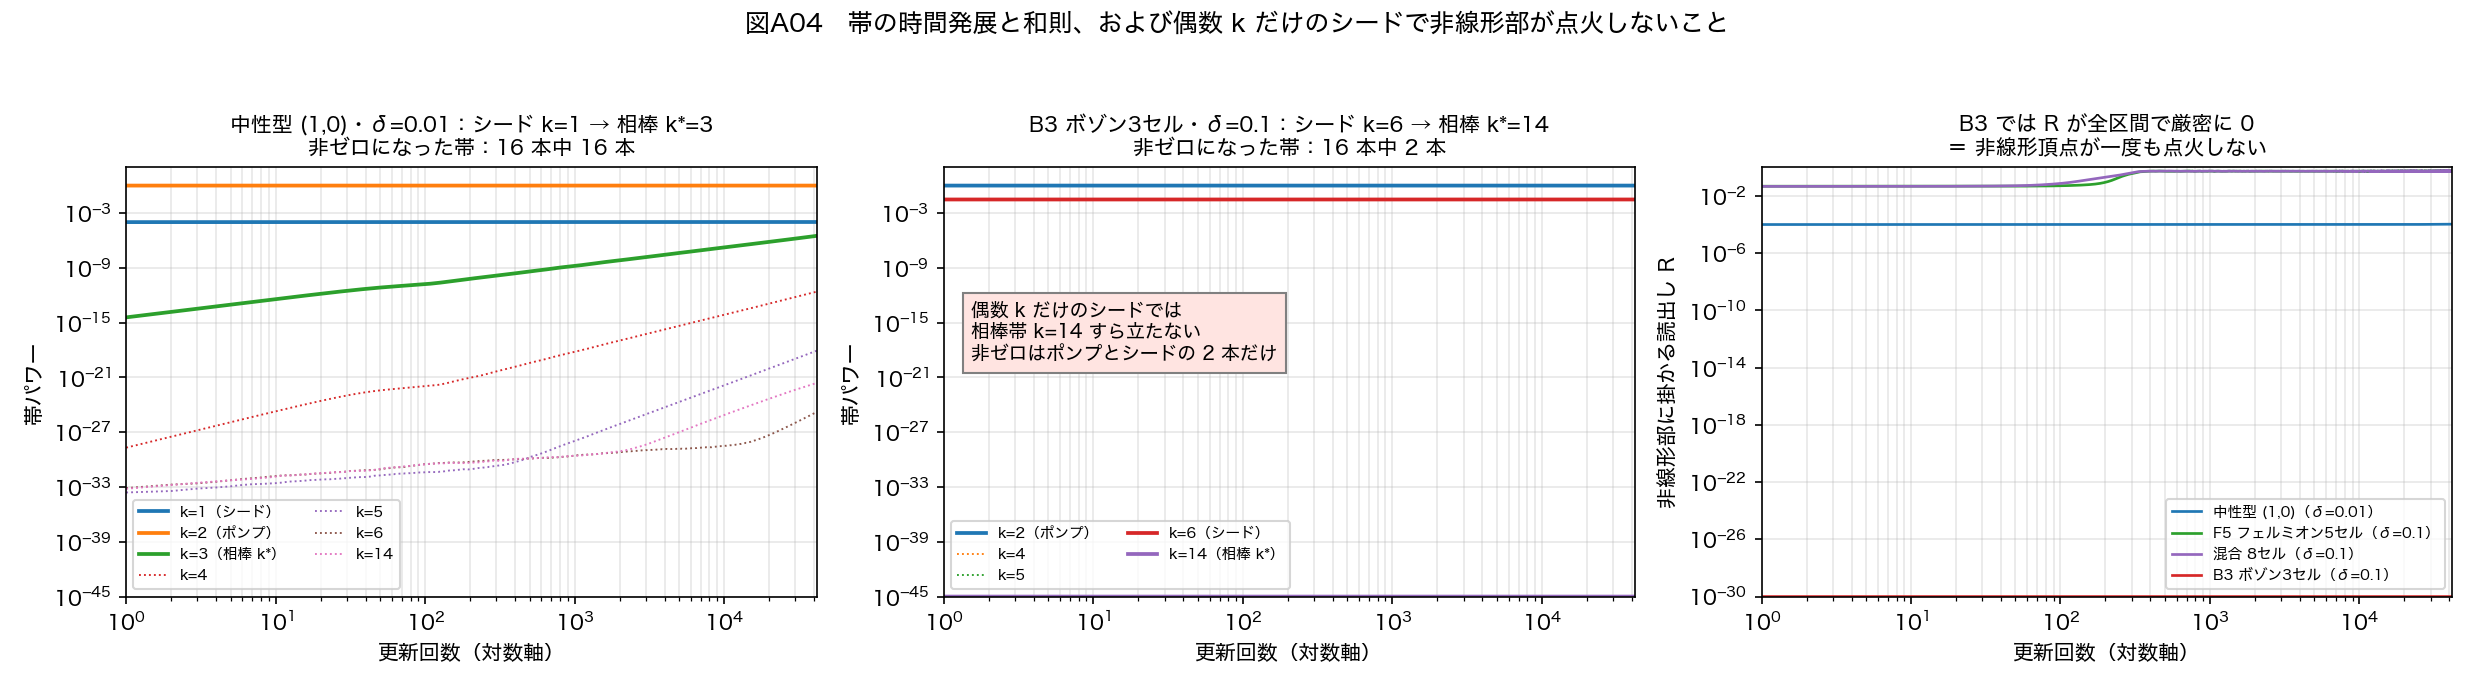
\includegraphics[keepaspectratio,alt={Figure 17　Growth by band. Left: the neutrino type, where the targeted partner band stands up. Middle: the even-band-only seed, where only 2 bands ever carry a wave. Right: the coefficient setting the interaction strength, identically zero for the even-band-only seed.}]{figA04_band_evolution_sumrule_v1.png}}

\textbf{Figure 17　Growth by band. Left: the neutrino type, where the
targeted partner band stands up. Middle: the even-band-only seed, where
only 2 bands ever carry a wave. Right: the coefficient setting the
interaction strength, identically zero for the even-band-only seed.}

\begin{figure}
\centering
\pandocbounded{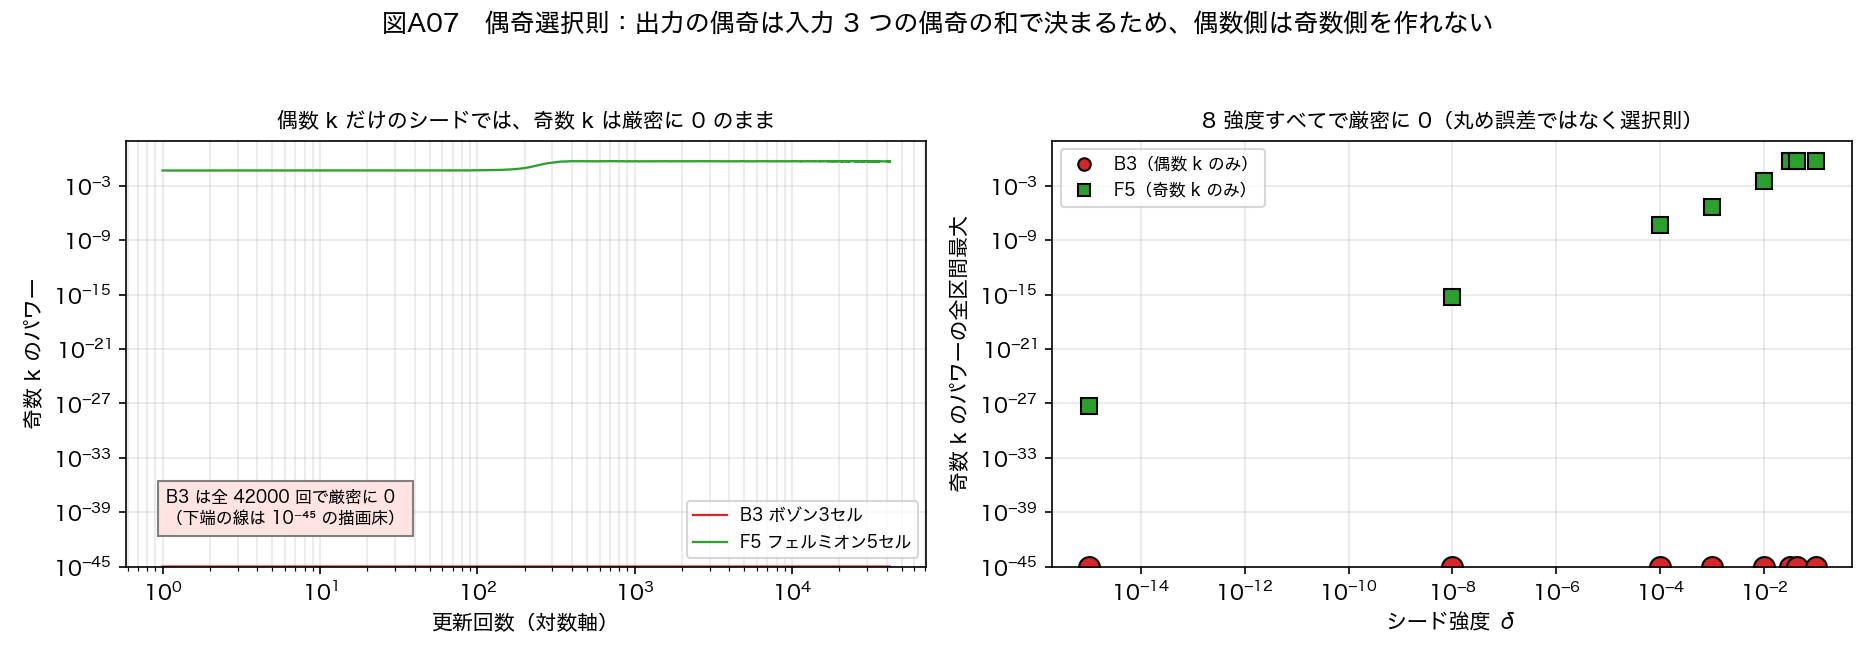
\includegraphics[keepaspectratio,alt={Figure 18　With a seed on even bands only, the odd bands stay exactly zero over the whole of 42000 updates and all 8 strengths.}]{figA07_parity_selection_rule_v1.png}}
\caption{Figure 18　With a seed on even bands only, the odd bands stay
exactly zero over the whole of 42000 updates and all 8 strengths.}
\end{figure}

\textbf{Figure 18　With a seed on even bands only, the odd bands stay
exactly zero over the whole of 42000 updates and all 8 strengths.}

\begin{center}\rule{0.5\linewidth}{0.5pt}\end{center}

\subsection{7) Time appears twice in this system: the order of updates
is not
time}\label{time-appears-twice-in-this-system-the-order-of-updates-is-not-time}

Two things that could be called time appear here. One is the
\textbf{count of updates kept from outside}, which is merely a serial
number we attach in order to run the experiment; it is not inside the
system. The other is the \textbf{clock the system reads from its own
state}, which exists only once the whole turns by a constant angle
without changing shape.

\textbf{These two must not be conflated.} No quantity named time is fed
into the dynamics of this system; what is fed in is only the update
procedure. Nevertheless, as the system develops, a tick of rotation
becomes readable from the relations among states. \textbf{Time is not
something given, but something that became readable.}

\subsubsection{Having a clock, its being constant, and its rate are
three different
things}\label{having-a-clock-its-being-constant-and-its-rate-are-three-different-things}

The number of updates at which the system becomes able to read its own
time, and the number at which the rate it reads settles to a constant
value, are different quantities.

\begin{itemize}
\tightlist
\item
  With seeds at eight locations and 4000 updates, \textbf{the rate does
  not settle for N ≥ 15} (the time has become readable)
\item
  Applying the phase cancellation of section 3, \textbf{the number of
  updates to settle falls from 15638 to 18, a factor of 870} (at
  strength 0.1, from 96 to 6)
\item
  The rate of the clock itself varies with condition. Of 132 runs,
  \textbf{67 deviated from the reference by more than 5\%}. The largest
  is the factor 9.9 at N = 4
\end{itemize}

\textbf{That the clock has been born does not mean the system keeps a
constant time.}
\pandocbounded{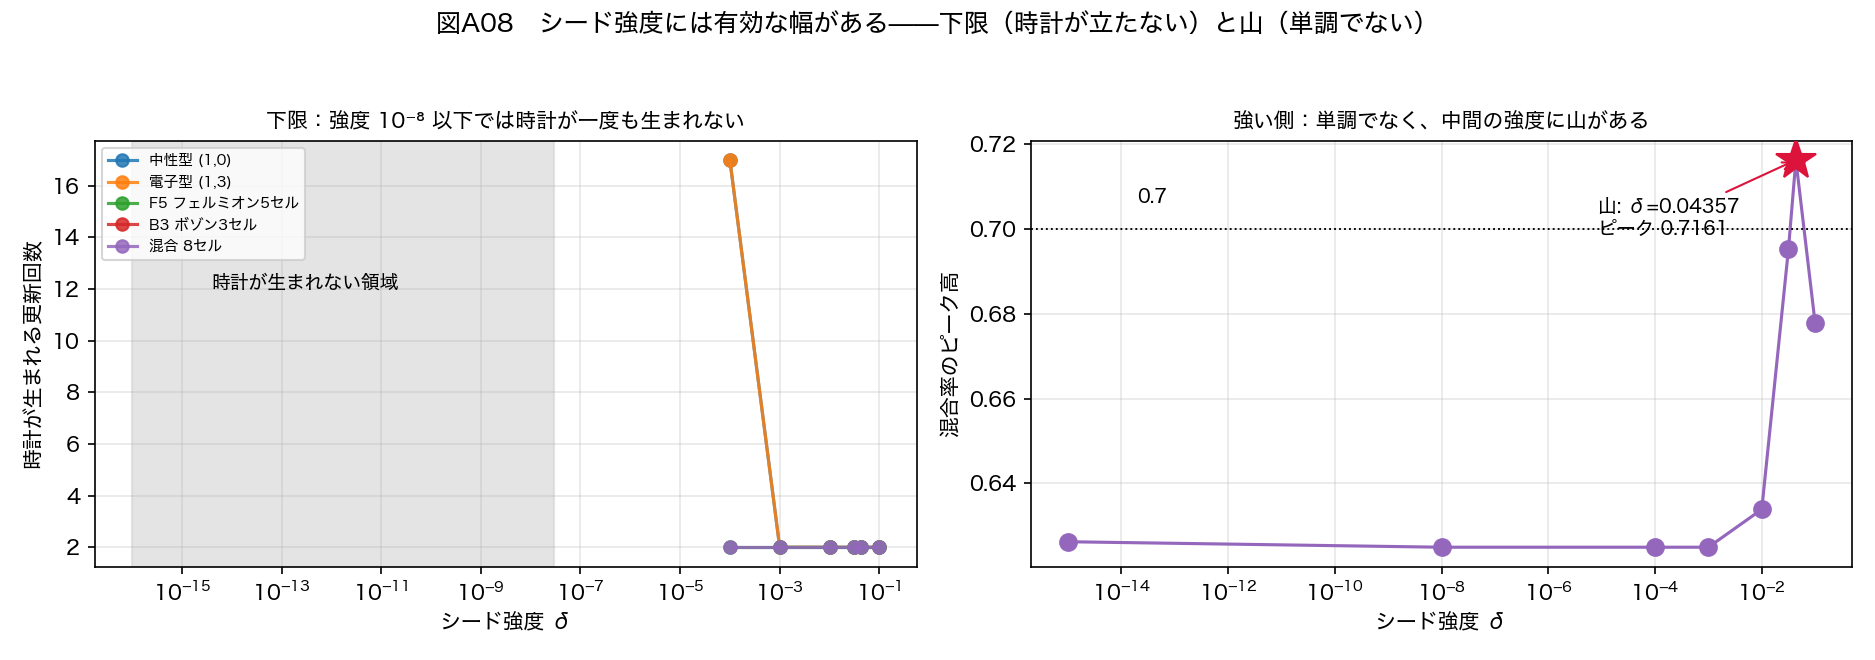
\includegraphics[keepaspectratio,alt={Figure 19　Updates at which the clock is born (left) and the peak of the mixing ratio (right). In the grey region on the left, no clock is born within the 42000 updates observed.}]{figA08_amplitude_window_v1.png}}

\textbf{Figure 19　Updates at which the clock is born (left) and the
peak of the mixing ratio (right). In the grey region on the left, no
clock is born within the 42000 updates observed.}

\begin{center}\rule{0.5\linewidth}{0.5pt}\end{center}

\subsection{8) The classification by greatest common divisor found in
the previous paper survives a change in the number of divisions of the
period}\label{the-classification-by-greatest-common-divisor-found-in-the-previous-paper-survives-a-change-in-the-number-of-divisions-of-the-period}

The previous paper found that, inside the background sea, the properties
of a wave depend not on the winding number of the second direction
itself but on \textbf{the greatest common divisor of that winding number
and the ``number of divisions of the period''}.

By the number of divisions of the period is meant, as in the description
of the system above, into how many parts one lap of the second direction
is divided. A winding number has meaning only as a remainder modulo that
number, so changing it should change which winding numbers fall into the
same class. The previous paper registered this as a question to be
tested. This paper tested it.

Re-running at the same number of divisions, 16, \textbf{all 62 values
agreed bit for bit} with the stored results of the previous paper.
Divisions of 8, 12 and 32 were then added, and \textbf{all 278 pairs
came out as predicted, with zero failures}.

The decisive case is the pair of winding numbers 1 and 3. If the
greatest common divisor governs, this pair should fall in the same class
at divisions 8, 16 and 32, and in \textbf{different classes at 12
alone}. Measurement gives \textbf{agreement to 14 digits} at 8, 16 and
32, and a \textbf{60\% difference at 12 alone}.
\pandocbounded{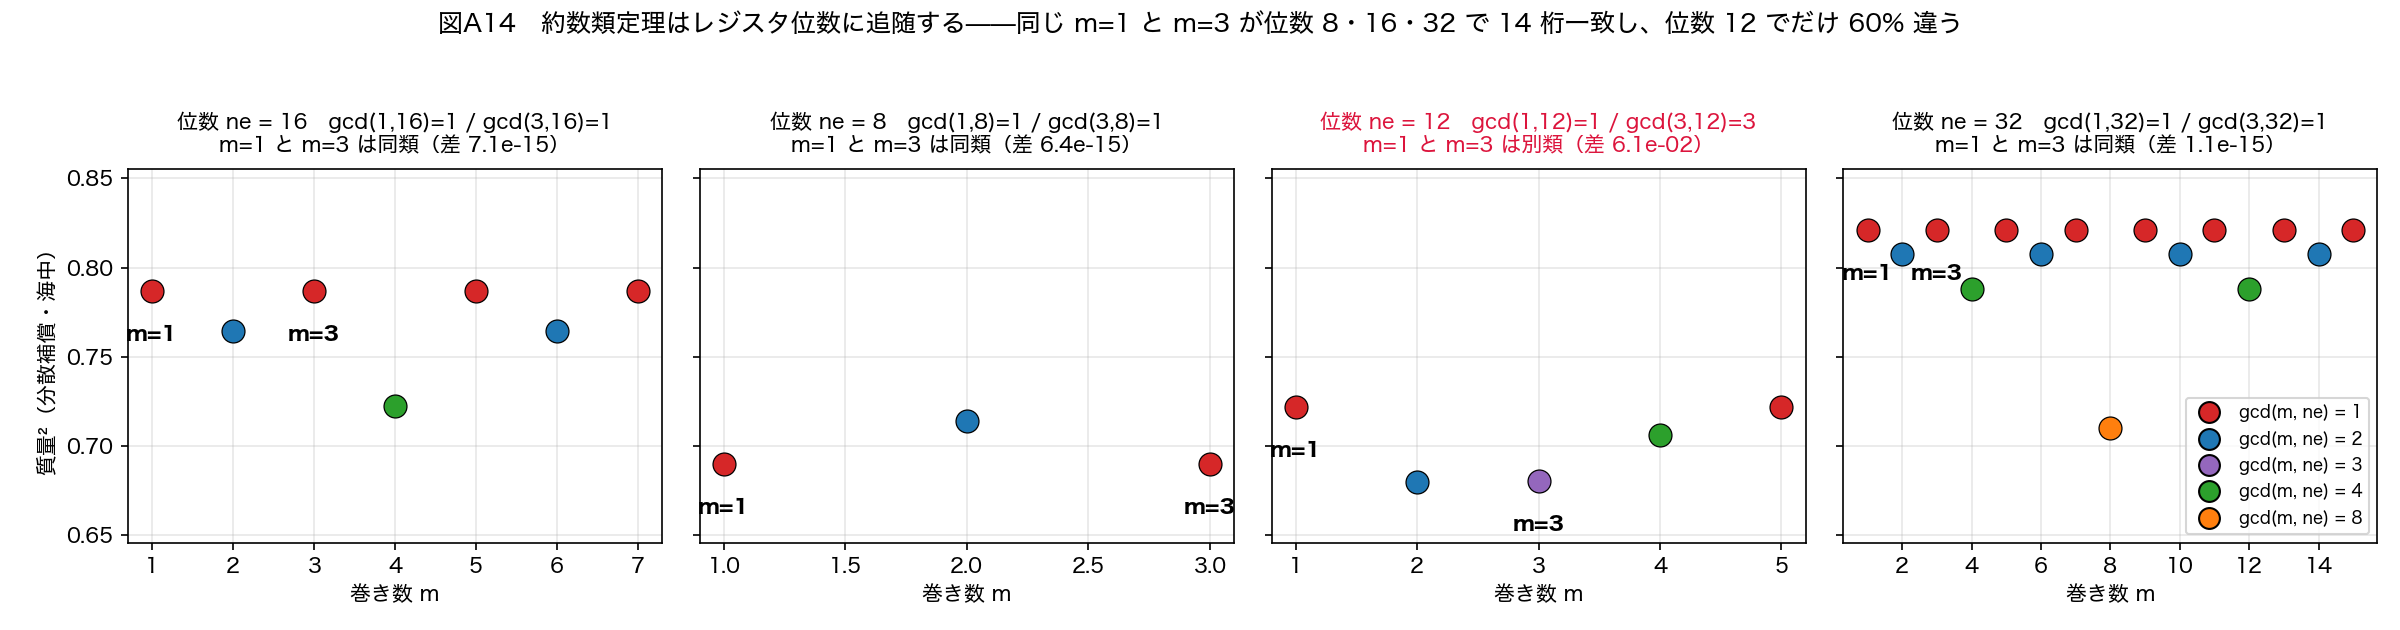
\includegraphics[keepaspectratio,alt={Figure 20　The test of changing the number of divisions of the period. Points of the same colour line up at the same height. Winding numbers 1 and 3 agree to 14 digits at divisions 8, 16 and 32, and differ by 60\% at 12 alone.}]{figA14_divisor_class_register_order_v1.png}}

\textbf{Figure 20　The test of changing the number of divisions of the
period. Points of the same colour line up at the same height. Winding
numbers 1 and 3 agree to 14 digits at divisions 8, 16 and 32, and differ
by 60\% at 12 alone.}

\begin{center}\rule{0.5\linewidth}{0.5pt}\end{center}

\subsection{Open questions}\label{open-questions}

\begin{enumerate}
\def\labelenumi{\arabic{enumi}.}
\tightlist
\item
  Whether the failure to build the initial state at N = 8 and N = 10 is
  structural or an artefact of the implementation cutting off after one
  attempt
\item
  Whether ``too weak a seed yields no particle-like wave'' is likewise
  an artefact of the observation time
\item
  The long run at strength 10⁻² with many seed locations. The saturation
  law (Figure 7) is drawn from 14 points; with those 2 added it becomes
  16. The exponent may shift, but the conclusion that a finite
  observation time must produce an apparent lower bound does not
\item
  Whether the classification by greatest common divisor also holds in
  the many-body system (section 8 was verified in the two-wave system)
\item
  A test changing the number of divisions of the first direction (16 in
  this experiment)
\item
  Measurement of the coefficient the interaction actually uses (the
  relation to the value 0.6972 of the previous paper is decided there)
\item
  Matching the 62 kinds of the previous paper against which location in
  this experiment corresponds to which particle
\end{enumerate}

The following go beyond the scope of this paper and are deferred to a
sequel.

\begin{enumerate}
\def\labelenumi{\arabic{enumi}.}
\setcounter{enumi}{7}
\item
  \textbf{An orthogonal experiment separating the run-up law from the
  saturation law.} The phase-cancellation experiment here fixed power
  and placement and varied the complex sum. Its orthogonal counterpart
  would \textbf{fix the sum and vary only the power}; the onset should
  be unchanged and only the finishing time should move. The same
  experiment would settle the ``sum versus sum of squares'' question of
  section 3, by including an arrangement whose sum is zero but whose sum
  of squares is not
\item
  \textbf{Falsification of the saturation law by extrapolation.} Freeze
  the exponent at the value from the existing 14 points, predict the
  finishing time for unmeasured strengths in advance, and go for the hit
  without refitting
\item
  \textbf{A formal audit of how far the system closes on relations
  alone.} For the three readouts used here (the plane and the third
  direction; bands and mixing ratio; the clock criterion), classify
  whether the inputs close on sets of relations alone, or whether
  quantities attached to individual points have crept in.

  \textbf{This must be taken in two stages.} Even if the readouts are
  confirmed to close on relations alone, that shows only that
  \textbf{the readout maps close on relations}, not that \textbf{the
  system itself runs on relations alone}. For the latter, the same audit
  is required of the construction of the initial state, the first half
  of the update, and the interaction.

  That is, one must check in turn, for each stage --- building the
  state, updating, interacting, reading out --- whether any quantity
  attached to a point itself has slipped in. This paper has not verified
  even the last of those stages.
\end{enumerate}

\begin{center}\rule{0.5\linewidth}{0.5pt}\end{center}

\section{Appendix　Full list of runs, figures and
programs}\label{appendix-full-list-of-runs-figures-and-programs}

This appendix was generated automatically by
\texttt{make\_paperA\_appendix\_v1.py}, which scans the folder. Nothing
in it was transcribed by hand. The Japanese edition carries the
identical tables; only the headings are translated here.

\subsection{Appendix A　The runs}\label{appendix-a-the-runs}

126 stored run files (NPZ), 1174 MB in total. Runs differing in seed
placement, seed strength, number of updates or resolution are counted as
different runs.

\begin{itemize}
\tightlist
\item
  40 conditions of the main experiment: 5 seed placements × 8 strengths
  (resolution 12, 42000 updates), all present
\item
  Resolution sweep N = 1\ldots20 for 4 conditions (no seed, neutrino
  type, electron type, mixed), 4000 updates
\item
  Reproduction controls, phase-cancelled arms and their replicate,
  resolution-4 runs, and long runs at 300000 updates
\end{itemize}

\subsection{Appendix B　The figures}\label{appendix-b-the-figures}

20 figures in the body; 462 per-run record figures; 41 contact sheets
used to inspect all of them. Naming is
\texttt{fig\_\textless{}seed\ placement\textgreater{}{[}\_T\textless{}updates\textgreater{}{]}{[}\_d\textless{}strength\textgreater{}{]}{[}\_rep-\textless{}tag\textgreater{}{]}\_\textless{}family\textgreater{}{[}\_N\textless{}resolution\textgreater{}{]}\_v2.png},
so any figure cited in the text is identified uniquely by its file name.

{\def\LTcaptype{none} % do not increment counter
\begin{longtable}[]{@{}
  >{\raggedright\arraybackslash}p{(\linewidth - 4\tabcolsep) * \real{0.3000}}
  >{\raggedright\arraybackslash}p{(\linewidth - 4\tabcolsep) * \real{0.3000}}
  >{\raggedleft\arraybackslash}p{(\linewidth - 4\tabcolsep) * \real{0.4000}}@{}}
\toprule\noalign{}
\begin{minipage}[b]{\linewidth}\raggedright
Family
\end{minipage} & \begin{minipage}[b]{\linewidth}\raggedright
Content
\end{minipage} & \begin{minipage}[b]{\linewidth}\raggedleft
Count
\end{minipage} \\
\midrule\noalign{}
\endhead
\bottomrule\noalign{}
\endlastfoot
4panel & space / number of competing planes / clock / cancellation
residue & 126 \\
mix & power per band and mixing ratio & 126 \\
ledger & map of the 128 locations, and growth at the targeted one &
78 \\
summary & per-resolution summary & 66 \\
birth\_matrix & the six criteria & 66 \\
\end{longtable}
}

\subsection{Appendix C　The programs}\label{appendix-c-the-programs}

Thirteen programs, plus five imported read-only. SHA-256 digests of
every one are listed in the Japanese edition and in
\texttt{論文A\_凍結マニフェスト\_v1.json}.

{\def\LTcaptype{none} % do not increment counter
\begin{longtable}[]{@{}
  >{\raggedright\arraybackslash}p{(\linewidth - 2\tabcolsep) * \real{0.5000}}
  >{\raggedright\arraybackslash}p{(\linewidth - 2\tabcolsep) * \real{0.5000}}@{}}
\toprule\noalign{}
\begin{minipage}[b]{\linewidth}\raggedright
Role
\end{minipage} & \begin{minipage}[b]{\linewidth}\raggedright
File
\end{minipage} \\
\midrule\noalign{}
\endhead
\bottomrule\noalign{}
\endlastfoot
Main experiment & \texttt{run\_nsweep\_three\_series\_v2.py},
\texttt{run\_tb\_nsweep\_1to20\_v1.py} \\
Additional seed placements &
\texttt{run\_missing\_seed\_sweeps\_T42000\_v1.py} \\
Phase-cancelled seed & \texttt{run\_phase\_balanced\_mixed\_v1.py},
\texttt{run\_phase\_balanced\_mixed\_grid\_v1.py} \\
Test of the number of divisions &
\texttt{run\_divisor\_class\_register\_order\_v1.py} \\
Recomputation and cross-check of every claimed number &
\texttt{aggregate\_paperA\_claims\_v1.py} \\
Figures & \texttt{make\_paperA\_figures\_v2.py},
\texttt{make\_paperA\_figures\_audit\_v1.py} \\
Closest approach to 0.6972 over all runs &
\texttt{probe\_alpha\_root\_closest\_approach\_v1.py} \\
Contact sheets for full visual inspection &
\texttt{make\_contact\_sheets\_v1.py} \\
This appendix & \texttt{make\_paperA\_appendix\_v1.py} \\
Long runs and resolution-4 runs &
\texttt{run\_stage4\_longtime\_orchestrator\_v1.py} \\
\end{longtable}
}

The dynamics itself (interaction, plane and third-direction readout,
band and mixing readout, clock criterion) and the two-wave map used in
section 8 are imported read-only and never modified. Each run verifies
their digests before and after.

\subsection{Appendix D　Pre-registrations, reports and
records}\label{appendix-d-pre-registrations-reports-and-records}

Pre-registration documents (predictions fixed before running), result
reports, the full-figure audit record, and the JSON files holding every
number.

\subsection{Appendix E　Results of the
cross-check}\label{appendix-e-results-of-the-cross-check}

Every number claimed was recomputed independently from the stored data
and checked mechanically against the existing records.

{\def\LTcaptype{none} % do not increment counter
\begin{longtable}[]{@{}
  >{\raggedright\arraybackslash}p{(\linewidth - 2\tabcolsep) * \real{0.5000}}
  >{\raggedright\arraybackslash}p{(\linewidth - 2\tabcolsep) * \real{0.5000}}@{}}
\toprule\noalign{}
\begin{minipage}[b]{\linewidth}\raggedright
Check
\end{minipage} & \begin{minipage}[b]{\linewidth}\raggedright
Result
\end{minipage} \\
\midrule\noalign{}
\endhead
\bottomrule\noalign{}
\endlastfoot
Onset and clock counts recomputed from stored data vs.~the records & 40
conditions, 0 mismatches \\
Number of locations occupied & agrees \\
Odd bands exactly zero for the even-band-only seed & maximum 0.0 \\
Run-up law & 9.8922 − 48.6108 × ln(complex sum), R² = 0.999868 \\
Same points organised by total power & R² = 0.992202 \\
The four phase-cancelled conditions & all as predicted \\
Reproduction of the previous paper (16 divisions) & 62 values, largest
discrepancy 0.0e+00 \\
Test of changing the number of divisions & 278 pairs, 0 failures \\
Law for the finishing time & ∝ (odd-band power)\^{}(−1.073), R² = 0.9960
(14 points) \\
\end{longtable}
}

\end{document}
